%!TEX root = ../main.tex

We apply our new methodology for designing compositional program analyses for dynamic languages to obtain a compositional symbolic execution engine for \jsil, an intermediate representation for JavaScript analysis~\cite{javert}.
%
%Much like JavaScript, \jsil does not exhibit the frame property~\cite{reynolds:lics:2002}, raising the issue of how to guarantee that the results of the analysis still hold when extending the initial state of the analysed program with a given arbitrary frame.
%
%The methodology has three steps: \dtag{1} designing an instrumented semantics of the language that exhibits the frame property, \dtag{2} designing the program  analysis on the instrumented semantics, and \dtag{3} linking the program analysis to the concrete semantics by describing the frames that can be safely added to the initial state.   
%
%The key innovation is to have the instrumented semantics as a proper interim stage in the design of the analysis, obtaining 
%more modular reasoning and substantially simpler proofs.
%
%For our symbolic analysis, 
We define a new, abstract semantics for \jsil,\footnote{We refer to the semantics as \emph{abstract} since it 
is parametric on a \jsil state signature. We are not doing abstract interpretation.} in the spirit %style % I think style is too strong because the citation is really abstract interpretation - it will be very confusing
 of~\cite{vanhorn:icfp:2010}, which we instantiate to obtain the concrete, instrumented, and symbolic semantics. 
This abstract semantics is the bedrock for both the formal development \emph{and} the implementation of the analysis. This approach has several benefits: it streamlines the formalism, avoiding redundancy; it makes the choices in the design of the instrumented and symbolic semantics explicit; and it leads to modular implementations, avoiding code duplication.
%
Full definitions and proofs are given in the~Appendix.

%In \S\ref{subsec:jsil:analysis:formalism}, we define an abstract semantics for 
%\jsil, which we then instantiate to obtain its concrete and symbolic semantics.
%In \S\ref{sex:formal:guarantees}, we present the formal guarantees of 
%our symbolic analysis, including: \dtag{i} a soundness result for the \jsil symbolic 
%execution, \dtag{ii} a guarantee of absence of false positives for bug-finding, \pmaxinline{Do we know what bug-finding is here?}
%\dtag{iii} a justification result for the lifting of analyses on compiled \jsil code back to JavaScript;
%and \dtag{iv} \polish{a verification result that precisely states the conditions 
%under which symbolic execution gives us verification guarantees.}
%Finally, in \S\ref{subsec:jsil:analysis:implementation}, we give a brief overview
%of our implementation. %in \rosette~\cite{Rosette1,Rosette2} NO NO NO! Burn the witch!

\vspace*{-0.2cm}
\subsection{\jsil Syntax and Abstract Semantics}\label{subsec:jsil:analysis:formalism}

\vspace*{-0.1cm}
\myparagraph{Syntax} \jsil is a simple goto language featuring top-level procedures and commands that operate on object heaps. It was purposefully designed to natively support the main dynamic features of JavaScript: extensible objects; dynamic property access; and dynamic procedure calls. The syntax of \jsil is shown below. 

\vspace{5pt}
\begin{display}{Syntax of the \jsil Language}{
\begin{tabular}{l}
	% $\jnumber \in \numbers$ \jspc  $\jbool \in \bools$ \jspc $\jstring \in \strings$  \jspc 
	% $\loc \in \locs$ \jspc $\jvar \in \jvars$ \jspc $\jtype \in \jtypes$ \\[0.1cm]
	 %
$\val \in \vals$ \defeq\ $\jnumber \! \mid \! \jbool \! \mid \! \jstring \! \mid \! {\small \jundefined} \! \mid \! {\small \jnull} \! \mid \! {\small \jempty} \! \mid \! \loc \! \mid \! \jtype \! \mid \!  \pid \! 
         \mid \! \jsillist{\val_i \mid_{i=0}^n} \! \mid \! \jsilset{\val_i \!\mid_{i=0}^n}$
   \\[0.1cm]
 %
  $\jsilexpr \in \exprs$ \defeq\ $\val \mid \jvar \mid \svar \mid \ominus\ \jsilexpr \mid \jsilexpr \binop{} \jsilexpr$
 \\[0.1cm]
%
$\bcmd \in \bcmds$ \defeq\ $\jsilskip \mid \jvar := \jsilexpr  \mid \jvar := \jsilnew() \mid \jvar := [\jsilexpr, \jsilexpr] \mid [\jsilexpr, \jsilexpr] := \jsilexpr $ \\
%
\hspace{0.02cm} $\mid \jsildelete(\jsilexpr, \jsilexpr) \mid \jvar := \hasfield(\jsilexpr, \jsilexpr) \mid \jvar := \getfields(\jsilexpr)$ \\[0.1cm]
% Commands
$\jcmd \in \cmds$ \defeq \ $ \bcmd \mid \goto \ i \mid  \ifgoto{\jsilexpr}{i}{j} \mid \jsilcall{\jvar}{\jsilexpr}{\jsilexpr_i\!\mid_{i=0}^n}{j}$ \\
\hspace{0.02cm} $ \mid \assume(\jsilexpr) \mid \jassert(\jsilexpr)$ \\[0.1cm]
%
$\proc \in \procs$ \defeq \ $\procedure{\pid}{\jvec{\jvar}}{\jvec{\jcmd}}$
\hspace{0.6cm}
$i, j \in \indexes$ $\semeq \mathbb{N} \cup \{ \retlab, \errlab \}$
 \end{tabular}}
\end{display}

\vspace{2pt}
\noindent \jsil \emph{values}, $\val \in \vals$, include numbers, booleans, strings, the special values $\jundefined$, $\jnull$, and $\jempty$, object locations~$\loc$, types~$\jtype$, procedure identifiers $\pid$, and lists and sets of values.
\jsil~\emph{expressions}, $\jsilexpr \in \exprs$, include \jsil values, \jsil program variables $\jvar$, various unary and binary operators, and symbolic variables $\svar$, introduced in this paper. Symbolic variables range over symbolic strings, numbers, booleans, and locations, denoted respectively by $\sstring$, $\snumber$, $\sbool$, and~$\sloc$.

%

\jsil \emph{basic commands} enable the manipulation of extensible objects and do not affect control flow. 
They include $\jsilskip$, variable assignment, object creation, property access, property assignment, property deletion, membership check, and property collection.
%, and a new command for symbolic variable creation. 
%
\jsil \emph{commands} include \jsil basic commands and control flow commands: conditional and unconditional gotos, dynamic procedure calls, and two new commands for symbolic reasoning, $\assume$ and $\jassert$.  %\footnote{\jsil also has a $\phi$-node assignment (cf.~\cite{javert}), supporting Static-Single-Assignment (SSA) \cite{SSA}. To avoid clutter, we omit it as it does not impact the reasoning.} 
The goto commands are intuitive: $\goto \ i$ jumps to the $i$-th command of the active procedure, and $\ifgoto{\jsilexpr}{i}{j}$ jumps to the $i$-th command if $\jsilexpr$ evaluates to $\jtrue$, and to the $j$-th otherwise. 
The dynamic procedure call $\jsilcall{\jvar}{\jsilexpr}{\jvec{\jsilexpr}}{j}$ evaluates  $\jsilexpr$ and $\jvec{\jsilexpr}$ to obtain the procedure identifier and arguments, respectively, executes the appropriate procedure with these arguments, and, in the end, assigns its return value to $\jvar$.
If the procedure raises an error, control is transferred to the $j$-th command; otherwise, it follows to the next command. 
%

A \jsil procedure is of the form $\procedure{\pid}{\jvec{\jvar}}{\jvec{\jcmd}}$, where $\pid$ is its identifier, $\jvec{\jvar}$ are its formal parameters, and its body ${\jvec{\jcmd}}$  is a sequence of \jsil commands. 
%\polish{When calling a procedure, any missing parameters are implicitly set to $\jundefined$.}
Procedures return via two dedicated indexes, $\retlab$ and $\errlab$, using two dedicated variables, $\retvar$ and $\errvar$. If a procedure reaches the $\retlab$ index, it returns normally with the return value denoted by $\retvar$; if it reaches $\errlab$, it returns an error, with the error value denoted by $\errvar$.
%
A \jsil program $\prog \in \progs$ is a set of top-level procedures, and its entry point is always the special procedure $\jsilmain$\hspace{-2pt}.


%
%\pmax{more modular, factor out. three for symbolic analysis}
\myparagraph{Abstract semantics} We design the abstract semantics to make the analysis, the proofs, and the implementations as modular as possible. At its core are the GetCell and GetDomain functions, which precisely pinpoint the way in which \jsil interacts with the heap, factoring out the common behaviour of \jsil basic commands. It also provides standard constructs for reasoning about symbolic values, whose concrete and instrumented semantics are trivial.

The abstract semantics is parametric on abstract states $\absstate \in \absstates$ and abstract values $\absval, \absprop, \absloc \in \absvals$. 
%For clarity, we use $\absprop$ and $\absloc$ to refer to abstract values denoting properties and locations, respectively.
%
Abstract states are assumed to have a store $\absstore: \jvars \partialmap \absvals$, mapping program variables $\jvar \in \jvars$ to abstract values. Stores are accessible via a store selector, $\absstate.\stosel$.
We use the special symbol $\none$ (read: none) to denote the absence of a property in an object, write $\setext{\absvals}{\none}$ for the set $\absvals \cup \{ \none \}$ and range over it using~$\iabsval$.
Abstract states expose the following functions and relations: 
\begin{description}
\setlength{\itemsep}{0.2em}
  \item[\jsil Expression Evaluation,] $\evalexpr{}(\absstore, \jsilexpr)$, which evaluates to the value of the \jsil expression $\jsilexpr$ under store $\absstore$. 

  %\item[Store Selector,] $\stosel : \absstates \rightarrow (\jvars \partialmap \absvals)$. The expression $\stosel(\absstate)$ evaluates to the store associated with a given  state $\absstate$. For clarity, we write $\absstate.\stosel$ instead of $\stosel(\absstate)$. 

  \item[Store Update,] $\stupdt{}(\absstate, \jvar, \absval)$, which denotes the state obtained from $\absstate$ 
             by updating the value of $\jvar$  to $\absval$ in $\absstate.\stosel$. 

  \item[Heap Allocation,] $\absalloc{}(\absstate)$, which evaluates to a pair consisting of a value denoting a fresh location and the new state that keeps track of that allocation. %
%             

   \item[Heap Update,] $\hpupdt{}(\absstate, \absloc, \absprop, \iabsval)$, denoting the state obtained from $\absstate$ by updating the value of property $\absprop$ of the object at location $\absloc$ to~$\iabsval$ or creating that property, in the
             case it does not exist.

  \item[GetCell,] $\absgetcellrule{}{\absstate, \jsilexpr_1, \jsilexpr_2}{\absstate', (\absloc, \absprop, \iabsval)}$, which retrieves the value associated with a given property of a given object. Formally, if $\absgetcellrule{}{\absstate, \jsilexpr_1, \jsilexpr_2}{\absstate', (\absloc, \absprop, \iabsval)}$ holds, 
          then: $\absloc$ denotes the location resulting from the evaluation of $\jsilexpr_1$, 
          $\absprop$~denotes the property name resulting from the evaluation of $\jsilexpr_2$, 
          $\iabsval$~denotes the value of the property $\absprop$ of the object at location $\absloc$, 
          and $\absstate'$ denotes a potential re-arrangement of $\absstate$ after property inspection (discussed in \S\ref{subsec:instrumented}). 
          %Observe the wide use of $\getcell$ in the abstract semantics of the basic commands (Figure~\ref{abs:sem:bcmds:fig}).
          %Also, $\getcell$ is non-deterministic and is, therefore, a relation.
            

               
             
  \item[GetDomain,] $\absgetdomainfun{}(\absstate, \jsilexpr)$, which denotes the 
           set of property names associated with the object at location resulting from the evaluation of $\jsilexpr$ 
           in $\absstate$. It is used in the \textsc{Property Collection} rule.
   
   %\item[Symbolic Value Creation,] $\absmakesymbolicrule{}{\jtype}$, which evaluates to a fresh  value of type $\jtype$.
   
   \item[Assumption,] $\absassume{}(\absstate, \jsilexpr)$, denoting the state obtained from $\absstate$ by stating that $\jsilexpr$ is assumed to evaluate to $\jtrue$. 
  
   \item[SAT Check,] $\abssat{}(\absstate, \jsilexpr)$, which evaluates to $\jtrue$ if the \jsil expression $\jsilexpr$ is satisfiable in the state~$\absstate$, and to $\jfalse$ otherwise.
             
\end{description}

\begin{figure}[t!]
{\scriptsize
\begin{mathpar}
  \inferrule[\textsc{Skip}]{}
	{ \absbsemrule{\absstate, \jsilskip}{\absstate}{}}  	
\qquad 
\inferrule[\textsc{Property Collection}]
  {
           \absval = \absgetdomainfun{}(\absstate, \jsilexpr)  
           \quad
           \absstate' =  \stupdt{}(\absstate, \jvar, \absval)
  }{\absbsemrule{\absstate, \jvar := \getfields(\jsilexpr)}{\absstate'}{}} 
\qquad 
\inferrule[\textsc{Assignment}]
  {
        \absstore = \absstate.\stosel
        \quad 
        \absval = \evalexpr{}(\absstore, \jsilexpr)
  }{\absbsemrule{\absstate, \jvar := \jsilexpr}{\stupdt{}(\absstate, \jvar, \absval)}{}} 
\\
\inferrule[\textsc{Object Creation}]
  { 
     (\loc, \absstate') = \absalloc{}(\absstate)   
      \qquad \absgetcellrule{}{\absstate', \loc, \protop}{\absstate'', -} \\\\ \absstate''' = \hpupdt{}(\absstate'', \loc, \protop, \jnull)
       }{\absbsemrule{\absstate, \jvar := \jsilnew()}{\stupdt{}(\absstate''', \jvar, \loc)}{}}
\qquad  
\inferrule[\textsc{Property Access}]
  { 
  	\absgetcellrule{}{\absstate, \jsilexpr_1, \jsilexpr_2}{\absstate', (-, -, \absval)}
  }{ \absbsemrule{\absstate, \jvar := [\jsilexpr_1, \jsilexpr_2]}{\stupdt{}(\absstate', \jvar, \absval)}{}}
%
\\
\inferrule[\textsc{Property Assignment}]
  {    
      \absgetcellrule{}{\absstate, \jsilexpr_1, \jsilexpr_2}{\absstate', (\absloc, \absprop, -)} 
      \\\\ \absstore = \absstate.\stosel \quad \absval = \evalexpr{}(\absstore, \jsilexpr_3)
  }{\absbsemrule{\absstate, [\jsilexpr_1, \jsilexpr_2] := \jsilexpr_3}{\hpupdt{}(\absstate', \absloc, \absprop, \absval)}{}} 
\qquad 
 \inferrule[\textsc{Property Deletion}]
  { 
        \absgetcellrule{}{\absstate, \jsilexpr_1, \jsilexpr_2}{\absstate', (\absloc, \absprop, \absval)}
  }{\absbsemrule{\absstate, \jsildelete(\jsilexpr_1, \jsilexpr_2)}{\hpupdt{}(\absstate', \absloc, \absprop, \none)}{}}
\\
\inferrule[\textsc{Member Check - True}]
  { 
     \absgetcellrule{}{\absstate, \jsilexpr_1, \jsilexpr_2}{\absstate', (-, -, \absval)}
     \\\\
    \absstate'' = \stupdt{}(\absstate', \jvar, \jtrue)
  }{\absbsemrule{\absstate, \jvar := \hasfield(\jsilexpr_1, \jsilexpr_2)}{\absstate''}{}}
 \qquad  
 \inferrule[\textsc{Member Check - False}]
  { 
     \absgetcellrule{}{\absstate, \jsilexpr_1, \jsilexpr_2}{\absstate', (-, -, \none)} 
     \\\\
    \absstate'' = \stupdt{}(\absstate', \jvar, \jfalse)
  }{\absbsemrule{\absstate, \jvar := \hasfield(\jsilexpr_1, \jsilexpr_2)}{\absstate''}{}}
%\inferrule[\textsc{Member Check - False}]
%  { 
%     \absgetcellrule{}{\absstate, \jsilexpr_1, \jsilexpr_2}{\absstate', (-, -, \none)} 
%     \\\\
%     \absstate'' =  \stupdt{}(\absstate', \jvar, \jfalse)
%  }{\absbsemrule{\absstate, \jvar := \hasfield(\jsilexpr_1, \jsilexpr_2)}{\absstate''}{}} \\
%  \inferrule[\textsc{Make Symbolic}]
%  { 
%     \absval = \absmakesymbolicrule{}{\absstate, \jtype}
%  }{\absbsemrule{\absstate, \jvar := \makesymbolic(\jtype)}{\stupdt{}(\absstate, \jvar, \absval)}{}}
\end{mathpar}}
\vspace*{-0.5cm}
 \captionsetup{format=nastyCaption}
\caption*{{\small Figure 3. Abstract semantics, basic commands: $\absbsemrule{\absstate, \bcmd}{\absstate'}{}$}}\label{abs:sem:bcmds:fig}
\vspace*{-0.4cm}
\end{figure}

%Assumption and the satisfiability check have trivial concrete semantic.

\noindent Transitions for basic commands have the form 
{\small $\absbsemrule{\absstate, \bcmd}{\absstate'}{}$}, meaning that the execution of the basic command 
$\bcmd$ in the state $\absstate$ results in the state $\absstate'$ (Fig.~3). 
%
To describe transitions of commands, we introduce \emph{execution modes}, $\mode$, and 
\emph{call stacks},~$\abscs$.  \jsil has two execution modes: 
$\top$, meaning the execution can proceed; and~$\bot$, meaning that the execution must stop due to an \emph{assert failure}. Call stacks are lists of tuples of the form $(\pid, \absstore, \jvar, i, j)$, where: 
$\pid$~is the identifier of the executing procedure;
$\absstore$~is the store of the procedure that called~$\pid$; 
$\jvar$~is the variable that will hold the return value of~$\pid$; %in~$\absstore$; 
and $i$ ($j$) is the index to which the control jumps when $\pid$ returns normally (with an error). 
%$i$ is the command index to which the control jumps when $\pid$ returns normally; 
%and $j$ is the command index to which the control jumps when $\pid$  returns an error. 
The \emph{initial call stack}, $\csmain$, is defined as {\small $[ (\jsilmain, \storeemp, \jsilout, 0, 0) ]$}, where ${\small\jsilout}$ holds the output of the entire program.  
Transitions for  commands have the form  {\small $\prog: \abssemrule{\absstate, \abscs, i}{\absstate', \abscs', j}{\mode}{\mode'}{}$}, 
meaning that, given a program~$\prog$, state~$\absstate$ and execution mode~$\mode$, the evaluation of the $i$-th command of the first procedure of %the call stack~
$\abscs$ generates 
the state~$\absstate'$, call stack $\abscs'$,  and the next command to be evaluated is the $j$-th command of the first procedure 
of~$\abscs'$, in execution mode~$\mode'$ (Fig.~4). 
For clarity, we keep the program implicit and write {\small $\ccmd{\abscs, i}$} to denote the $i$-th command of the first procedure of $\abscs$.

% We write $\ccmd{i}$ when $\prog$ and $\abscs$ are implicit.
%\vspace{-3pt}
\myparagraph{Notation} In the following, we denote a function with an empty domain by $\hemp$, and for a function $f : A \partialmap B$, we denote its domain extension/update by $f[a \mapsto b]$ %, denoting the heap $\heap$ extended with $\heap(\loc,\jstring) = \val$;
and the union of two functions with disjoint compatible domains by $f_1 \dunion f_2$. 

\begin{table*}[t!]
\centering 
{\scriptsize \begin{tabular}{@{}c@{}ccc@{}c@{}}\toprule
\multicolumn{3}{c}{{\it Concrete Execution: successful (left); failing (right)}} & &  \emph{Instrumented Execution}  \\
%\cmidrule{1-3} \cmidrule{5-5}
%\emph{Successful}  &  & \emph{Failing}  &   &       \\
\cmidrule{1-3} \cmidrule{5-5}
{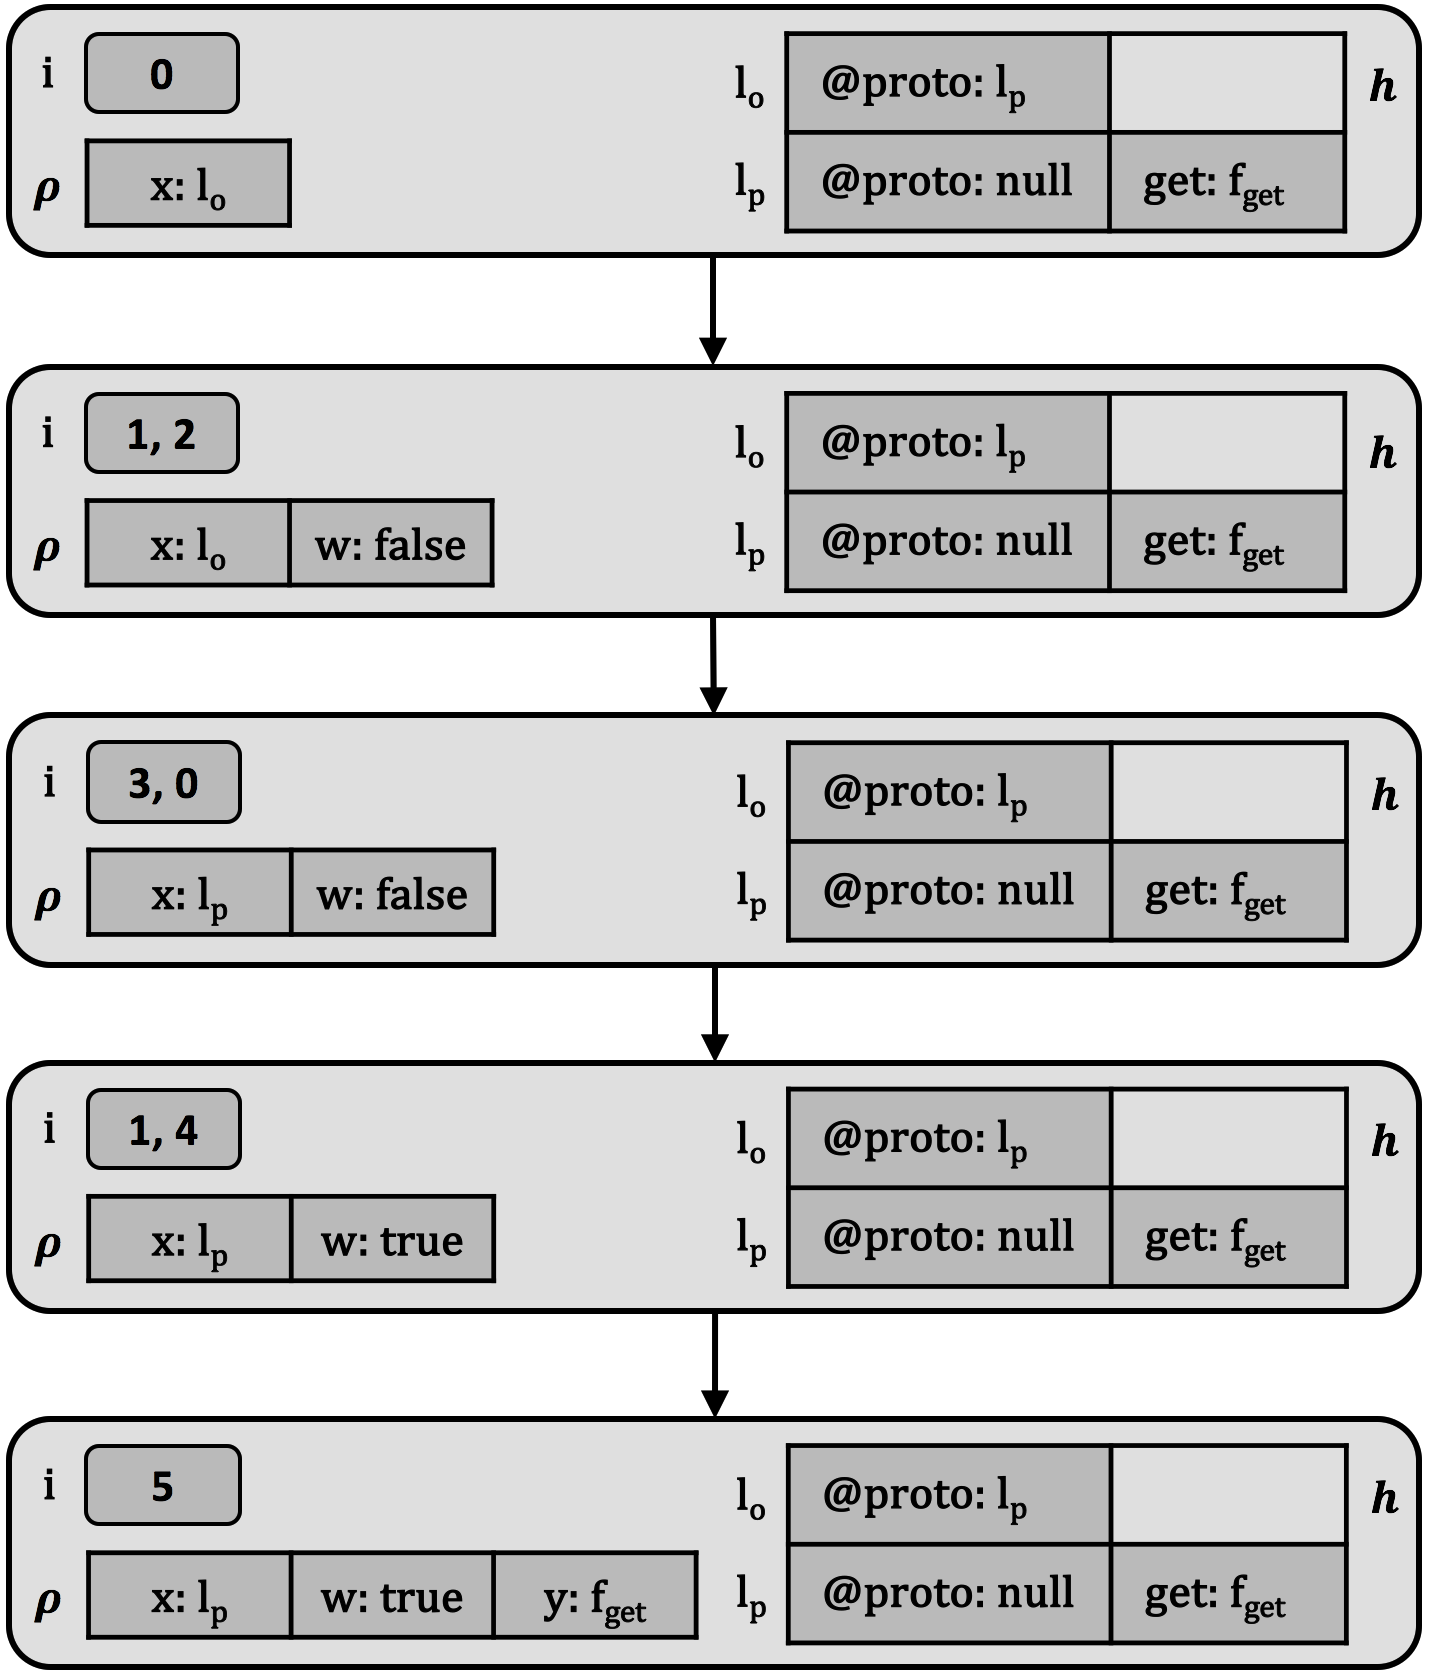
\includegraphics[width=0.305\textwidth,valign=T]{figures/conc_exec.png}} & & 
{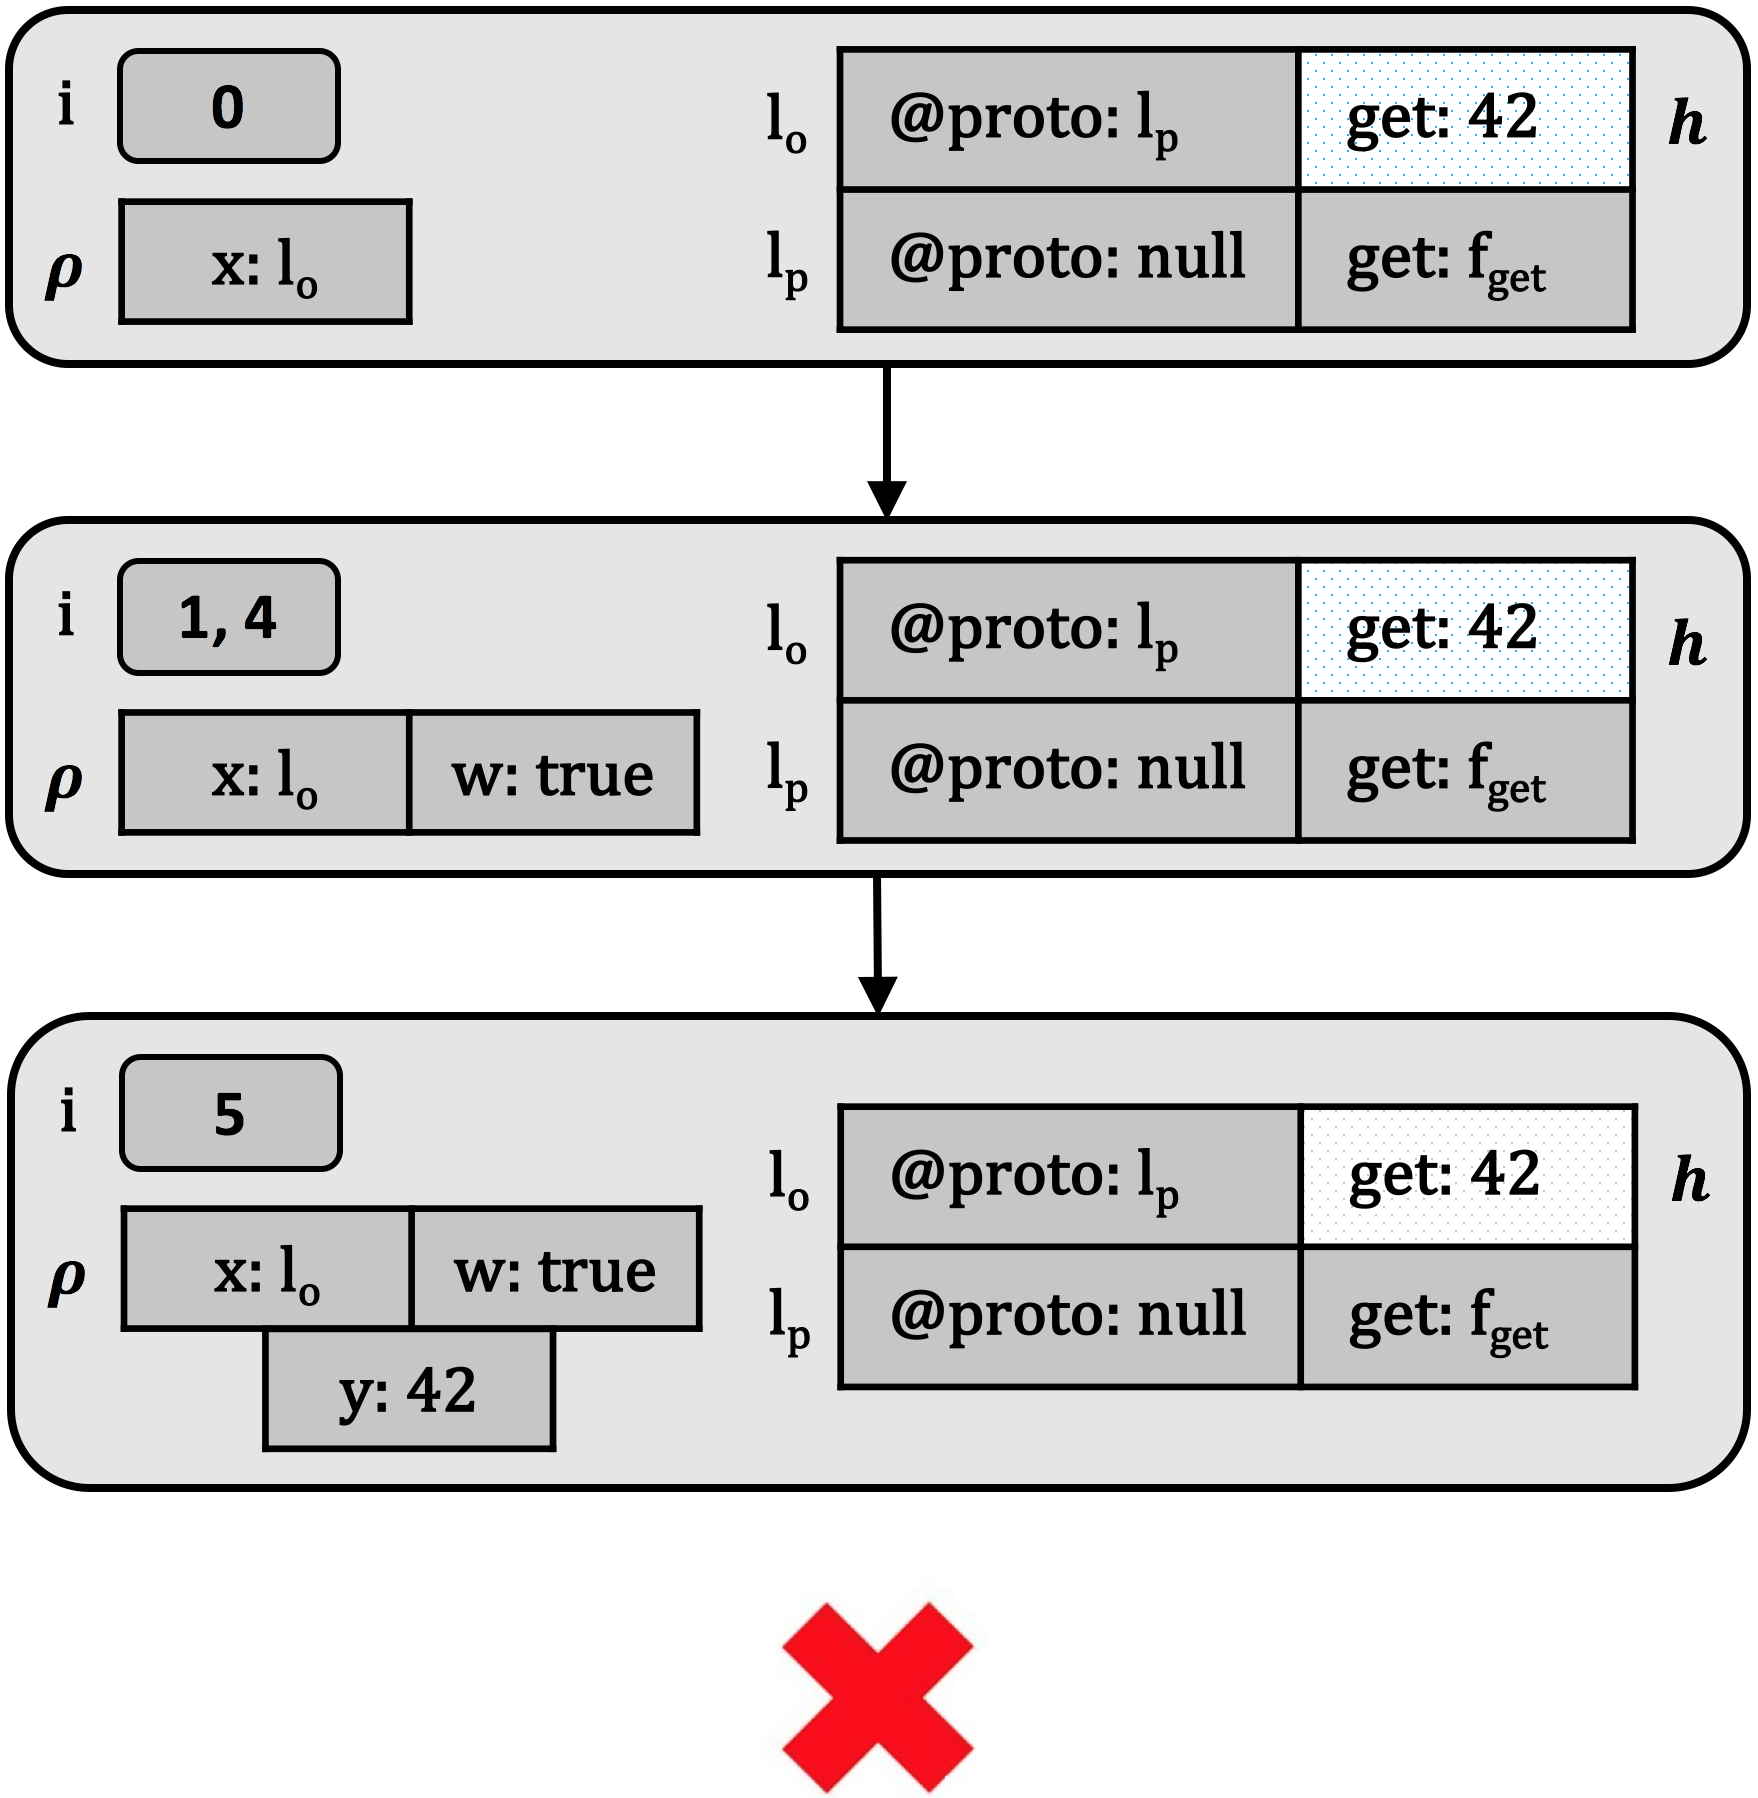
\includegraphics[width=0.265\textwidth,valign=T]{figures/conc_wrong_exec.png}} & & 
{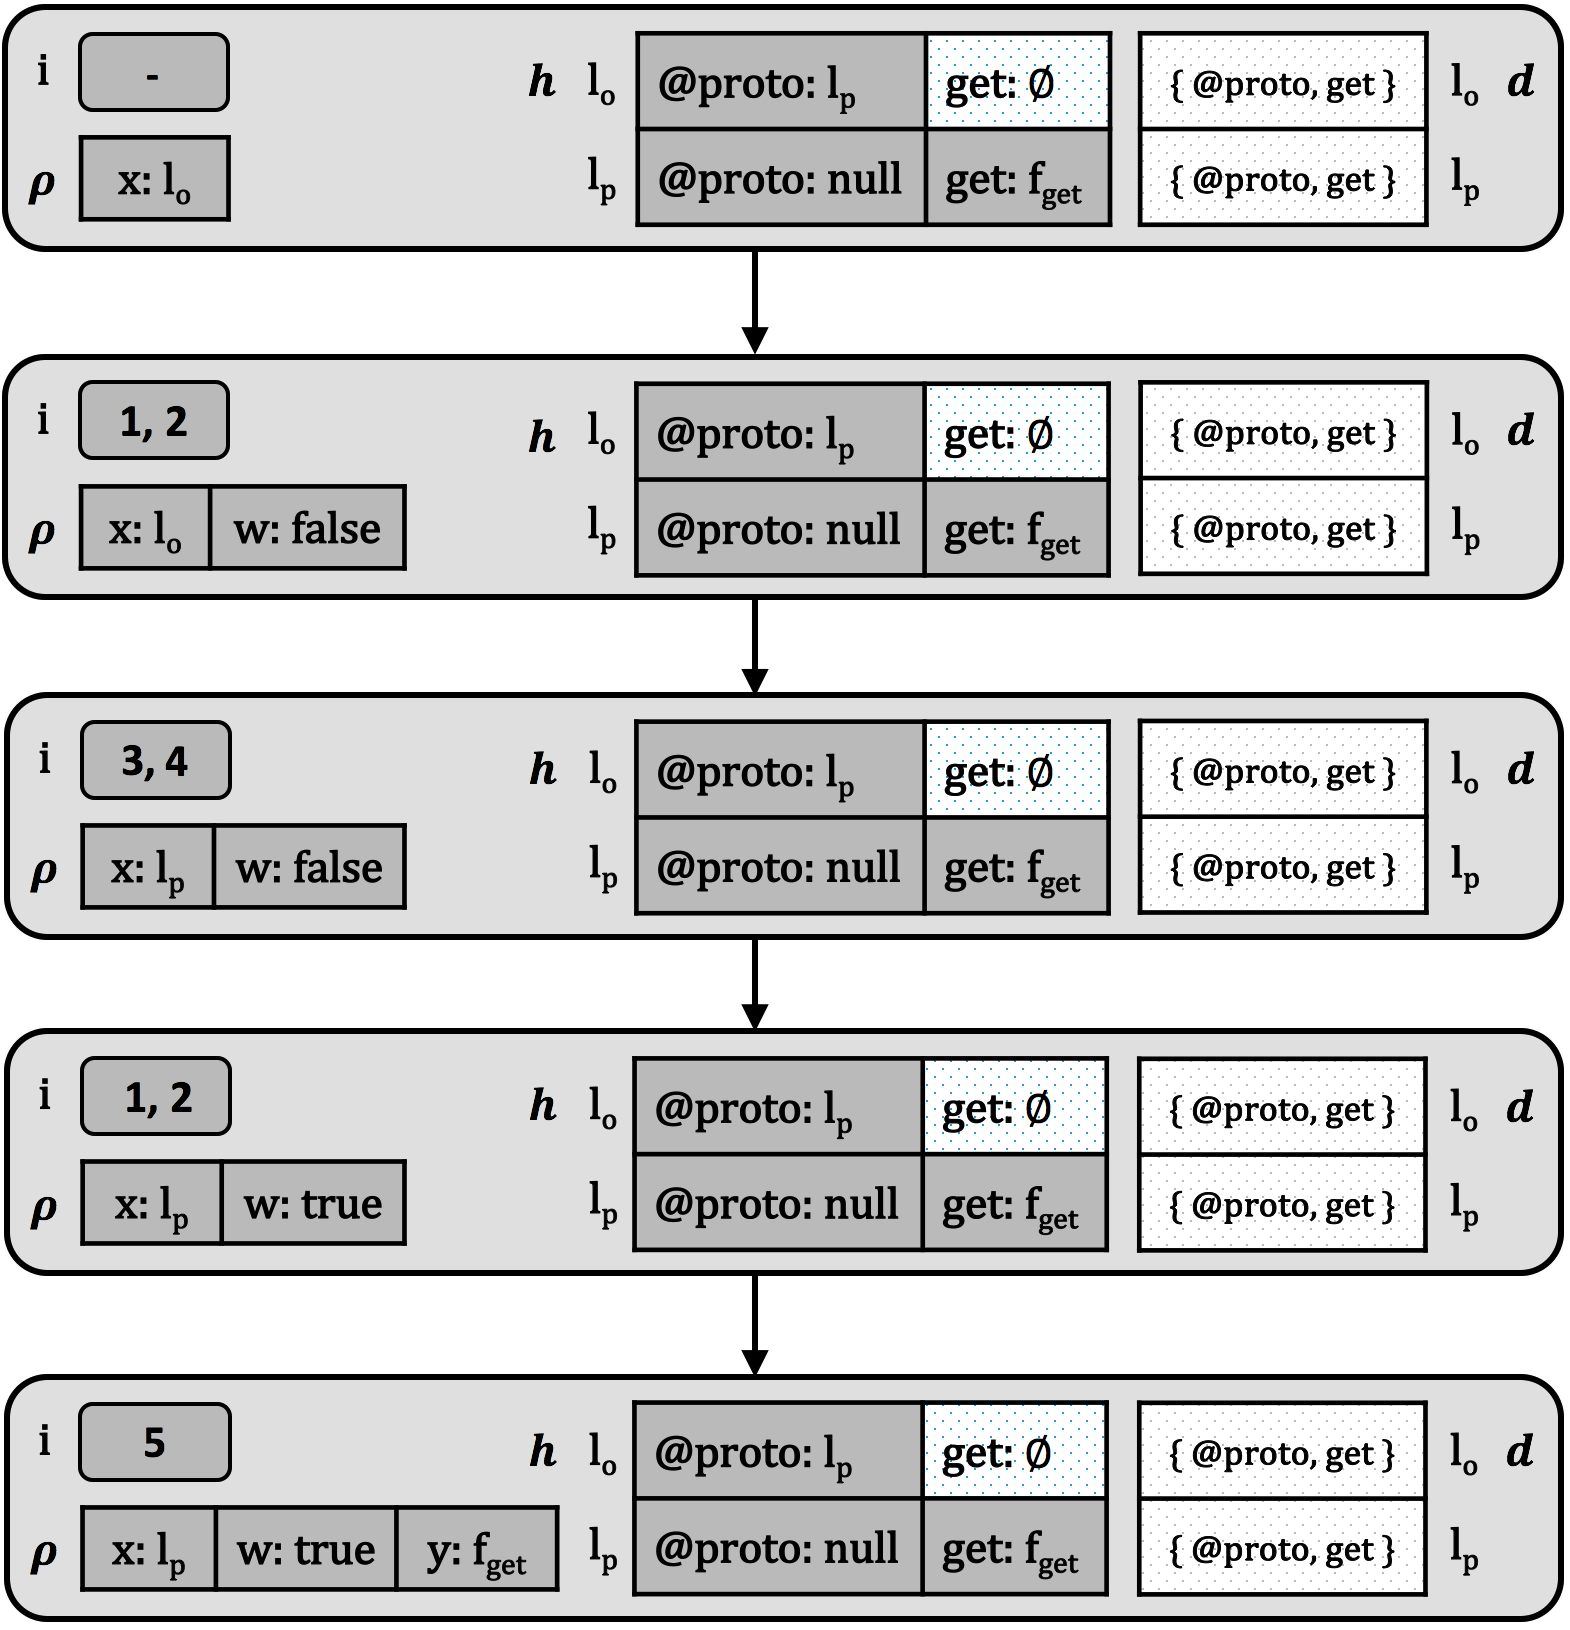
\includegraphics[width=0.347\textwidth,valign=T]{figures/inst_exec.png}}  \\  
\bottomrule
\end{tabular}}
\vspace{2pt}
\caption{Concrete vs. instrumented execution\label{example:symb:states:vs:assertions}}
\vspace*{-0.9cm}
\end{table*}

\begin{figure}[t!]
{\scriptsize
\begin{mathpar} 
\inferrule[\textsc{Basic Command}]
   { 
     \ccmd{\abscs, i} = \bcmd 
     \quad
     \absbsemrule{\absstate, \bcmd}{\absstate'}{} 
   }{\abssemrule{\absstate, \abscs, i}{\absstate', \abscs, i{+}1}{\top}{\top}{}}
   \and 
     \inferrule[\textsc{Goto}]
   { 
   \ccmd{\abscs, i} = \goto \, j \quad}
   {\abssemrule{\absstate, \abscs, i}{\absstate, \abscs, j}{\top}{\top}{}}
   \\
   %
  \inferrule[\textsc{Cond. Goto - True}]
   { \ccmd{\abscs, i} =  \ifgoto{\jsilexpr}{j}{k} 
     %\quad
     %   \absval = \evalexpr{}(\absstate.\stosel, \jsilexpr)
     %   \quad 
     %\absstate' = \absassume{}(\absstate, \jsilexpr) 
   }
   {\abssemrule{\absstate, \abscs, i}{\absassume{}(\absstate, \jsilexpr), \abscs, j}{\top}{\top}{}}
  %
  \qquad
  % 
  \inferrule[\textsc{Cond. Goto - False}]
   { \ccmd{\abscs, i} =  \ifgoto{\jsilexpr}{j}{k} 
      %\quad 
       % \absval = \evalexpr{}(\absstate.\stosel, \jsilexpr)
       % \quad 
      %\absstate' = \absassume{}(\absstate, \neg\jsilexpr) 
   }
   {\abssemrule{\absstate, \abscs, i}{\absassume{}(\absstate, \neg\jsilexpr), \abscs, k}{\top}{\top}{}}
  %
  \\
   %
   \inferrule[\textsc{Normal Return}]
   {
       \abscs = (-, \absstore', \jvar, i, -) :: \abscs'  
       \quad 
       \absstore = \absstate.\stosel
       \\\\
       \absstate' = \stupdt{}(\absstate[\stosel \mapsto \absstore'], \jvar, \absstore(\retvar))
   }  
   {\abssemrule{\absstate, \abscs, \retlab}{\absstate', \abscs', i}{\top}{\top}{}}
     %
   \qquad 
   %
      \inferrule[\textsc{Error Return}]
   { 
       \abscs = (-, \absstore', \jvar, -, j) :: \abscs'
       \quad 
       \absstore = \absstate.\stosel
       \\\\
        \absstate' = \stupdt{}(\absstate[\stosel \mapsto \absstore'], \jvar, \absstore(\errvar))
   }  
   {\abssemrule{\absstate, \abscs, \errlab}{\absstate', \abscs', j}{\top}{\top}{}}
      \\
    \inferrule[\textsc{Procedure Call}]
   { 
    \ccmd{\abscs, i} =   \jsilcall{\jvar}{\jsilexpr}{\jsilexpr_i \mid_{i = 0}^{n}}{j}
     \quad
     \absstore = \absstate.\stosel 
     \quad
    \evalexpr{}(\absstore, \jsilexpr) =  \pid' 
        \quad
     \args(\pid') = \jsillist{\jvar_1, ..., \jvar_{m}} 
      \\\\
      \absval_i = \evalexpr{}(\absstore, \jsilexpr_i) \mid_{i = 0}^{n} 
     \and
      \absval_i = \jundefined \mid_{i = n+1}^{m}  
      \and 
      \absstore' = [ \jvar_i \mapsto \absval_i \mid_{i = 0}^{m}]
   }
   {\abssemrule{\absstate, \abscs, i}{\absstate[\stosel \mapsto \absstore'],  (\pid', \absstore, \jvar, i{+}1, j) :: \abscs, 0}{\top}{\top}{}}
    \\
%
\inferrule[\textsc{Assume}]
  { 
      \ccmd{i}  = \assume(\jsilexpr) 
      \\\\ 
     \absstate' = \absassume{}(\absstate, \jsilexpr) 
  }{\abssemrule{\absstate, \abscs, i}{\absstate', \abscs, i{+}1}{\top}{\top}{}} 
\qquad
\inferrule[\textsc{Assert - True}]
  { 
      \ccmd{\abscs, i}  = \jassert(\jsilexpr)
      \\\\ 
      %\absstore = \absstate.\stosel
      %\quad
      %\absval = \evalexpr{}(\absstore, \jsilexpr)
      % \\\\
       \abssat{}(\absstate, \neg \jsilexpr) = \jfalse
  }{\abssemrule{\absstate, \abscs, i}{\absstate, \abscs, i{+}1}{\top}{\top}{}} 
\qquad 
\inferrule[\textsc{Assert - False}]
  { 
      \ccmd{\abscs, i}  = \jassert(\jsilexpr)
      \\\\ 
      %\absstore = \absstate.\stosel
      %\quad
      %  \absval = \evalexpr{}(\absstore, \jsilexpr)
      % \\\\
      \abssat{}(\absstate, \neg \jsilexpr) = \jtrue
  }{\abssemrule{\absstate, \abscs, i}{\absstate, \abscs, i}{\top}{\bot}{}} 
 \end{mathpar}}
 \vspace*{-0.52cm}
 \captionsetup{format=nastyCaption}
\caption*{{\small Figure 4. Abstract semantics, commands: $\abssemrule{\absstate, \abscs, i}{\absstate', \abscs', j}{\mode}{\mode'}{}$}}\label{abs:sem:cmds:fig}
\vspace*{-0.6cm}
\end{figure}

\vspace*{-0.2cm}
\subsection{\jsil Concrete Semantics}
\label{subsec:concr}
A \jsil concrete state $\jstate$ is a pair $(\heap, \store)$, consisting of a heap and a store. 
A heap, $\heap \in \heaps$, is a partial function mapping pairs of  object locations and property names (strings) to \jsil values.
A store, $\store \in \stores$, maps program variables to \jsil values. 
In the following, we denote a heap cell by $\hcell{\loc}{\jstring}{\val}$, meaning that $\heap(\loc, \jstring) = \val$.

We instantiate the abstract semantics for the concrete case by providing the appropriate definitions 
for the required abstractions.
%, noting that abstract values are instantiated to\jsil values extended with the property absence indicator $\none$.
We write $\absbsemrule{\jstate, \bcmd}{\jstate'}{\concrete}$ for the concrete semantic 
judgement for \jsil basic commands and $\abssemrule{\jstate, \cs, i}{\jstate', \cs', j}{\mode}{\mode'}{\concrete}$ 
for \jsil commands. 

The instantiation of the \jsil abstract semantics to the concrete case is straightforward: if an object \jsinline|l| has property \jsinline|p|, GetCell returns the associated value, and $\none$ otherwise; GetDomain returns the set of properties of a given object;
heap allocation returns a fresh object location without changing the state;
the rules for store update and positive heap update are standard; and 
the negative heap update removes the given property of a given object from the heap.
Note that the positive and negative heap update rules are not applicable at the same time, as $\val$ cannot be equal to $\none$. 

\smallskip
\begin{display}{Selected Concrete Semantics Rules}
\text{
{\scriptsize
\begin{mathpar} 
%  \inferrule[\textsc{Expression Evaluation}]
%  {}{\evalexpr{\concrete}(\store, \val) = \val \qquad 
%  	\evalexpr{\concrete}(\store, \jvar) = \store(\jvar) \qquad 
%	\evalexpr{\concrete}(\store, \ominus \jsilexpr) = \semop{\ominus} \ \evalexpr{c}(\store, \jsilexpr) \qquad
%	\evalexpr{\concrete}(\store, \jsilexpr_1 \oplus \jsilexpr_2) = \evalexpr{c}(\store, \jsilexpr_1) \ \semop{\oplus} \ \evalexpr{c}(\store, \jsilexpr_2)}
%  \\
    %
        \inferrule[\textsc{GetCell - Found}]
   { 
         \loc = \evalexpr{\concrete}(\store, \jsilexpr_1) 
        \quad 
         p = \evalexpr{\concrete}(\store, \jsilexpr_2) 
        \\\\
       \heap = - \, \uplus \, (\loc, p) \mapsto \val
       \quad 
       r = (\loc, p, \val)
        }{  \absgetcellrule{\concrete}{(\heap, \store), \jsilexpr_1, \jsilexpr_2}{(\heap, \store), r}}
        \qquad
    \inferrule[\textsc{GetCell - Not Found}]
   { 
         \loc = \evalexpr{\concrete}(\store, \jsilexpr_1) 
        \quad 
         p = \evalexpr{\concrete}(\store, \jsilexpr_2) 
        \\\\
       (\loc, p) \not\in \domain(\heap)
       \quad 
       r = (\loc, p, \none)
        }{  \absgetcellrule{\concrete}{(\heap, \store), \jsilexpr_1, \jsilexpr_2}{(\heap, \store), r}}
  %
  \\
  \inferrule[\textsc{GetDomain}]
   { 
       \loc = \evalexpr{\concrete}(\store, \jsilexpr) 
      \quad (\loc,-) \notin \domain (\heap') \\\\
       \heap = \heap' \, \uplus \, \big((\loc, p_i) \mapsto \val_i \big)\mid_{i = 0}^m  
       }{  \absgetdomainfun{\concrete}((\heap, \store), \jsilexpr) \semeq \jsilset{p_1, ..., p_m}}
  %
 %
 \quad 
    \inferrule[\textsc{Heap Alloc.}]
   { %\loc \text{ fresh } 
       \jstate = (\heap, -) \\\\
       %
       (\loc, -) \not\in \domain(\heap)
   }{
   \absalloc{c}(\absstate) =  (\loc, \jstate)}
   \quad
   \inferrule[\textsc{Store Update}]
   { 
         \store' = \store[\jvar \mapsto \val]
   }{  \stupdt{\concrete}((\heap, \store), \jvar, \val) =  (\heap, \store')}
   \\ 
       \inferrule[\textsc{Positive Heap Update}]
   { 
         \heap' = \heap[(\loc, p) \mapsto \val]
         %\quad 
      %  {\color{red} \val \neq \none}
   }{  \hpupdt{\concrete}((\heap, \store), \loc, p, \val) \semeq  (\heap', \store)}
 \qquad
       \inferrule[\textsc{Negative Heap Update}]
   { 
         \heap = \heap' \dunion (\loc, p) \mapsto -
   }{  \hpupdt{\concrete}((\heap, \store), \loc, p, \none) \semeq  (\heap', \store)}
%   \\\\
%      \inferrule[\textsc{Expr - SymbVar}]
%   {\svar \in \svars \text{ is of type } \jtype \\\\
%   \val \in \vals \text{ is of type } \jtype
%   }{\evalexpr{\concrete}(-, \svar) \semeq \val}
    
%  \inferrule[\textsc{Assume}]
%   {
%       \evalexpr{\concrete}(\jstate.\stosel, \jsilexpr) = \jtrue
%   }{  \absassume{\concrete}(\jstate, \jsilexpr) \semeq  \jstate }
%  	\and
%    \inferrule[\textsc{Check Sat}]
%   {
%        \jbool = \evalexpr{\concrete}(\jstate.\stosel, \jsilexpr) 
%   }{  \abssat{\concrete}(\jstate, \jsilexpr) \semeq \jbool}
  \end{mathpar}
  }}
 \end{display}

%The remaining rules can be seen in the Appendix.

%\jfs{
%\begin{itemize}
%   %\item mention the missing rules
%   \item explain the two getcell rules 
%   %\item explain the symbols that are not defined
%\end{itemize}
%}


\begin{wrapfigure}{R}{0.13\textwidth}
\vspace*{-0.2cm}
{\footnotesize
\hspace*{-0.47cm} $\mathtt{1\quad w := \hasfield(x, \litstring{get})}$ \\[-0.08cm]
\hspace*{-0.47cm} $\mathtt{2\quad \ifgoto{w}{5}{3}}$ \\[-0.08cm]
\hspace*{-0.47cm} $\mathtt{3\quad x := [x, \litstring{\protop}] }$ \\ [-0.08cm]
\hspace*{-0.47cm} $\mathtt{4\quad \ifgoto{x = \jnull}{\errlab}{1}}$ \\[-0.08cm]
\hspace*{-0.47cm} $\mathtt{5\quad y := [x, \litstring{get}]}$ \\[-0.08cm]
\hspace*{-0.47cm} $\mathtt{6\quad \jsilcall{z}{y}{}{\errlab}}$ 
}
\vspace*{-0.2cm}
%{\hspace*{-1cm}{\mbox{\caption{\jsil Example 1\label{jsil:example:frame}}}}}
\end{wrapfigure}



\smallskip
\myparagraph{Example: Frame}
The \jsil concrete semantics does not satisfy the frame property. 
We illustrate this with the program on the right, which 
looks for the property $\litstring{get}$ in the 
prototype chain of the object bound to $\mathtt{x}$, reads the value of that 
property, and calls the procedure whose identifier is bound to that value. 
The program terminates successfully when run from the state 
described in the top left corner of Table~\ref{example:symb:states:vs:assertions}. However, if we extend the initial state with the frame $(\loc_o, \litstring{get}) \mapsto 42$, 
as shown in the second column of Table~\ref{example:symb:states:vs:assertions}, the procedure 
call fails, as $42$ is not a procedure identifier. 

\vspace*{-0.2cm}
\subsection{\jsil Instrumented Semantics}\label{subsec:instrumented}


%Our instrumented semantics explicitly keeps track of properties that are not present in a given object, using ideas from~\cite{gardner:popl:2012,javert}.

Compositional analyses must reason about programs given partial state information.
This is particularly challenging for languages that do not observe the frame property.
We approach this problem by first designing an instrumented version of the language semantics that \emph{does} 
observe the frame property. 
%
To achieve this, the \jsil instrumented semantics keeps track of both the present \emph{and the absent} properties of a given object, 
using ideas from~\cite{gardner:popl:2012,javert}.

An instrumented state $\istate$ is a triple $(\iheap, \idom, \store)$ consisting of an instrumented heap, 
a domain table, and a store. 
%
An instrumented heap, $\iheap \in \iheaps : \locs \partialmap \strings \partialmap \setext{\vals}{\none}$, 
differs from a concrete heap in that it can map object properties to $\none$, explicitly declaring their absence. 
We refer to those cells as \emph{$\none$-cells} (read: none-cells). 
%
A domain table, $\idom : \locs \partialmap \vals$, maps object locations to sets of properties that the corresponding objects may have, whereas all other properties are \emph{known to be} absent. If $\idom(\loc)$ is defined and if $p \not\in \idom(\loc)$, then we know that the object at $\loc$ \emph{does not have} the property~$p$, and that that property \emph{cannot} be framed on. In contrast, any properties in $\idom(\loc)$ that are not in the heap can be safely framed on. Also, if we have that $(\loc, p) \in \domain(\iheap)$, then it holds that $p \in \idom(\loc)$.
On the other hand, if $\idom(\loc)$ is not defined, then all properties of the object at $\loc$ that are not in the heap \emph{can be} safely framed~on.

%We also know that all of the 
%properties of that object that are in the heap are also in $\idom(\loc)$.
%In this way, we implicitly keep track of an infinite number of absent properties.

We instantiate the abstract semantics to the instrumented case. 
We write $\absbsemrule{\istate, \bcmd}{\istate'}{\instrumented}$ for the instrumented semantic 
judgement for basic commands, and $\abssemrule{\istate, \cs, i}{\istate', \cs', j}{\mode}{\mode'}{\instrumented}$ 
for~commands. The omitted rules coincide with the concrete case. 

\begin{display}{Selected Instrumented Semantics Rules}
\text{
{\scriptsize
\begin{mathpar} 
     \inferrule[\textsc{Heap Update}]
   { 
         \istate = (\iheap, \idom, \store) 
         \quad
         \iheap' = \iheap[(\loc, p) \mapsto \ival]
   }{  \hpupdt{\instrumented}(\istate, (\loc, p), \ival) =  (\iheap', \idom, \store) }
   \and
      \inferrule[\textsc{GetCell - Found}]
   { 
        \istate = (\iheap, -, \store) 
        \quad
         \loc = \evalexpr{\concrete}(\store, \jsilexpr_1) 
      \\\\
         p = \evalexpr{\concrete}(\store, \jsilexpr_2) 
         \quad 
       \iheap = - \, \uplus \, (\loc, p) \mapsto \ival
        }{  \absgetcellrule{\instrumented}{\istate, \jsilexpr_1, \jsilexpr_2}{\istate, (\loc, p, \ival)}}
        \\
 % 
     \inferrule[\textsc{GetCell - Not Found}]
   { 
        \loc = \evalexpr{\concrete}(\store, \jsilexpr_1) 
        \quad 
         p = \evalexpr{\concrete}(\store, \jsilexpr_2) 
         \quad
         p \not\in \idom(\loc) 
         \quad
         \iheap' = \iheap \dunion (\loc, p) \mapsto \none
         \quad
         \idom' = \idom[\loc \mapsto \idom(\loc) \cup \jsilset{p}]
            }{  \absgetcellrule{\instrumented}{(\iheap, \idom, \store), \jsilexpr_1, \jsilexpr_2}{(\iheap', \idom', \store), (\loc, p, \none)}}
  %
  \\
  \inferrule[\textsc{GetDomain}]
   { 
       \loc = \evalexpr{\concrete}(\store, \jsilexpr) 
      \and
       \iheap = \iheap' \, \uplus \, \big((\loc, p_i) \mapsto - \big)\mid_{i = 0}^m  
        \and
        %
          (\loc,-) \notin \domain (\iheap')  
        \\\\
          \jsilset{p_1, ..., p_m} = \idom(\loc)
          \and
        \forall_{0 \leq i \leq n} \, \val_i \neq \none 
         \and 
           \forall_{n < i \leq m} \, \val_i = \none 
   }{  \absgetdomainfun{\instrumented}((\iheap, \idom, \store), \jsilexpr) \semeq \jsilset{p_1, ..., p_n}}
 %
 % 
 \end{mathpar}}}
 \end{display}
 
 
\setcounter{figure}{4}   
\begin{figure*}[!t]
\centering
\begin{tabular}{c||c}
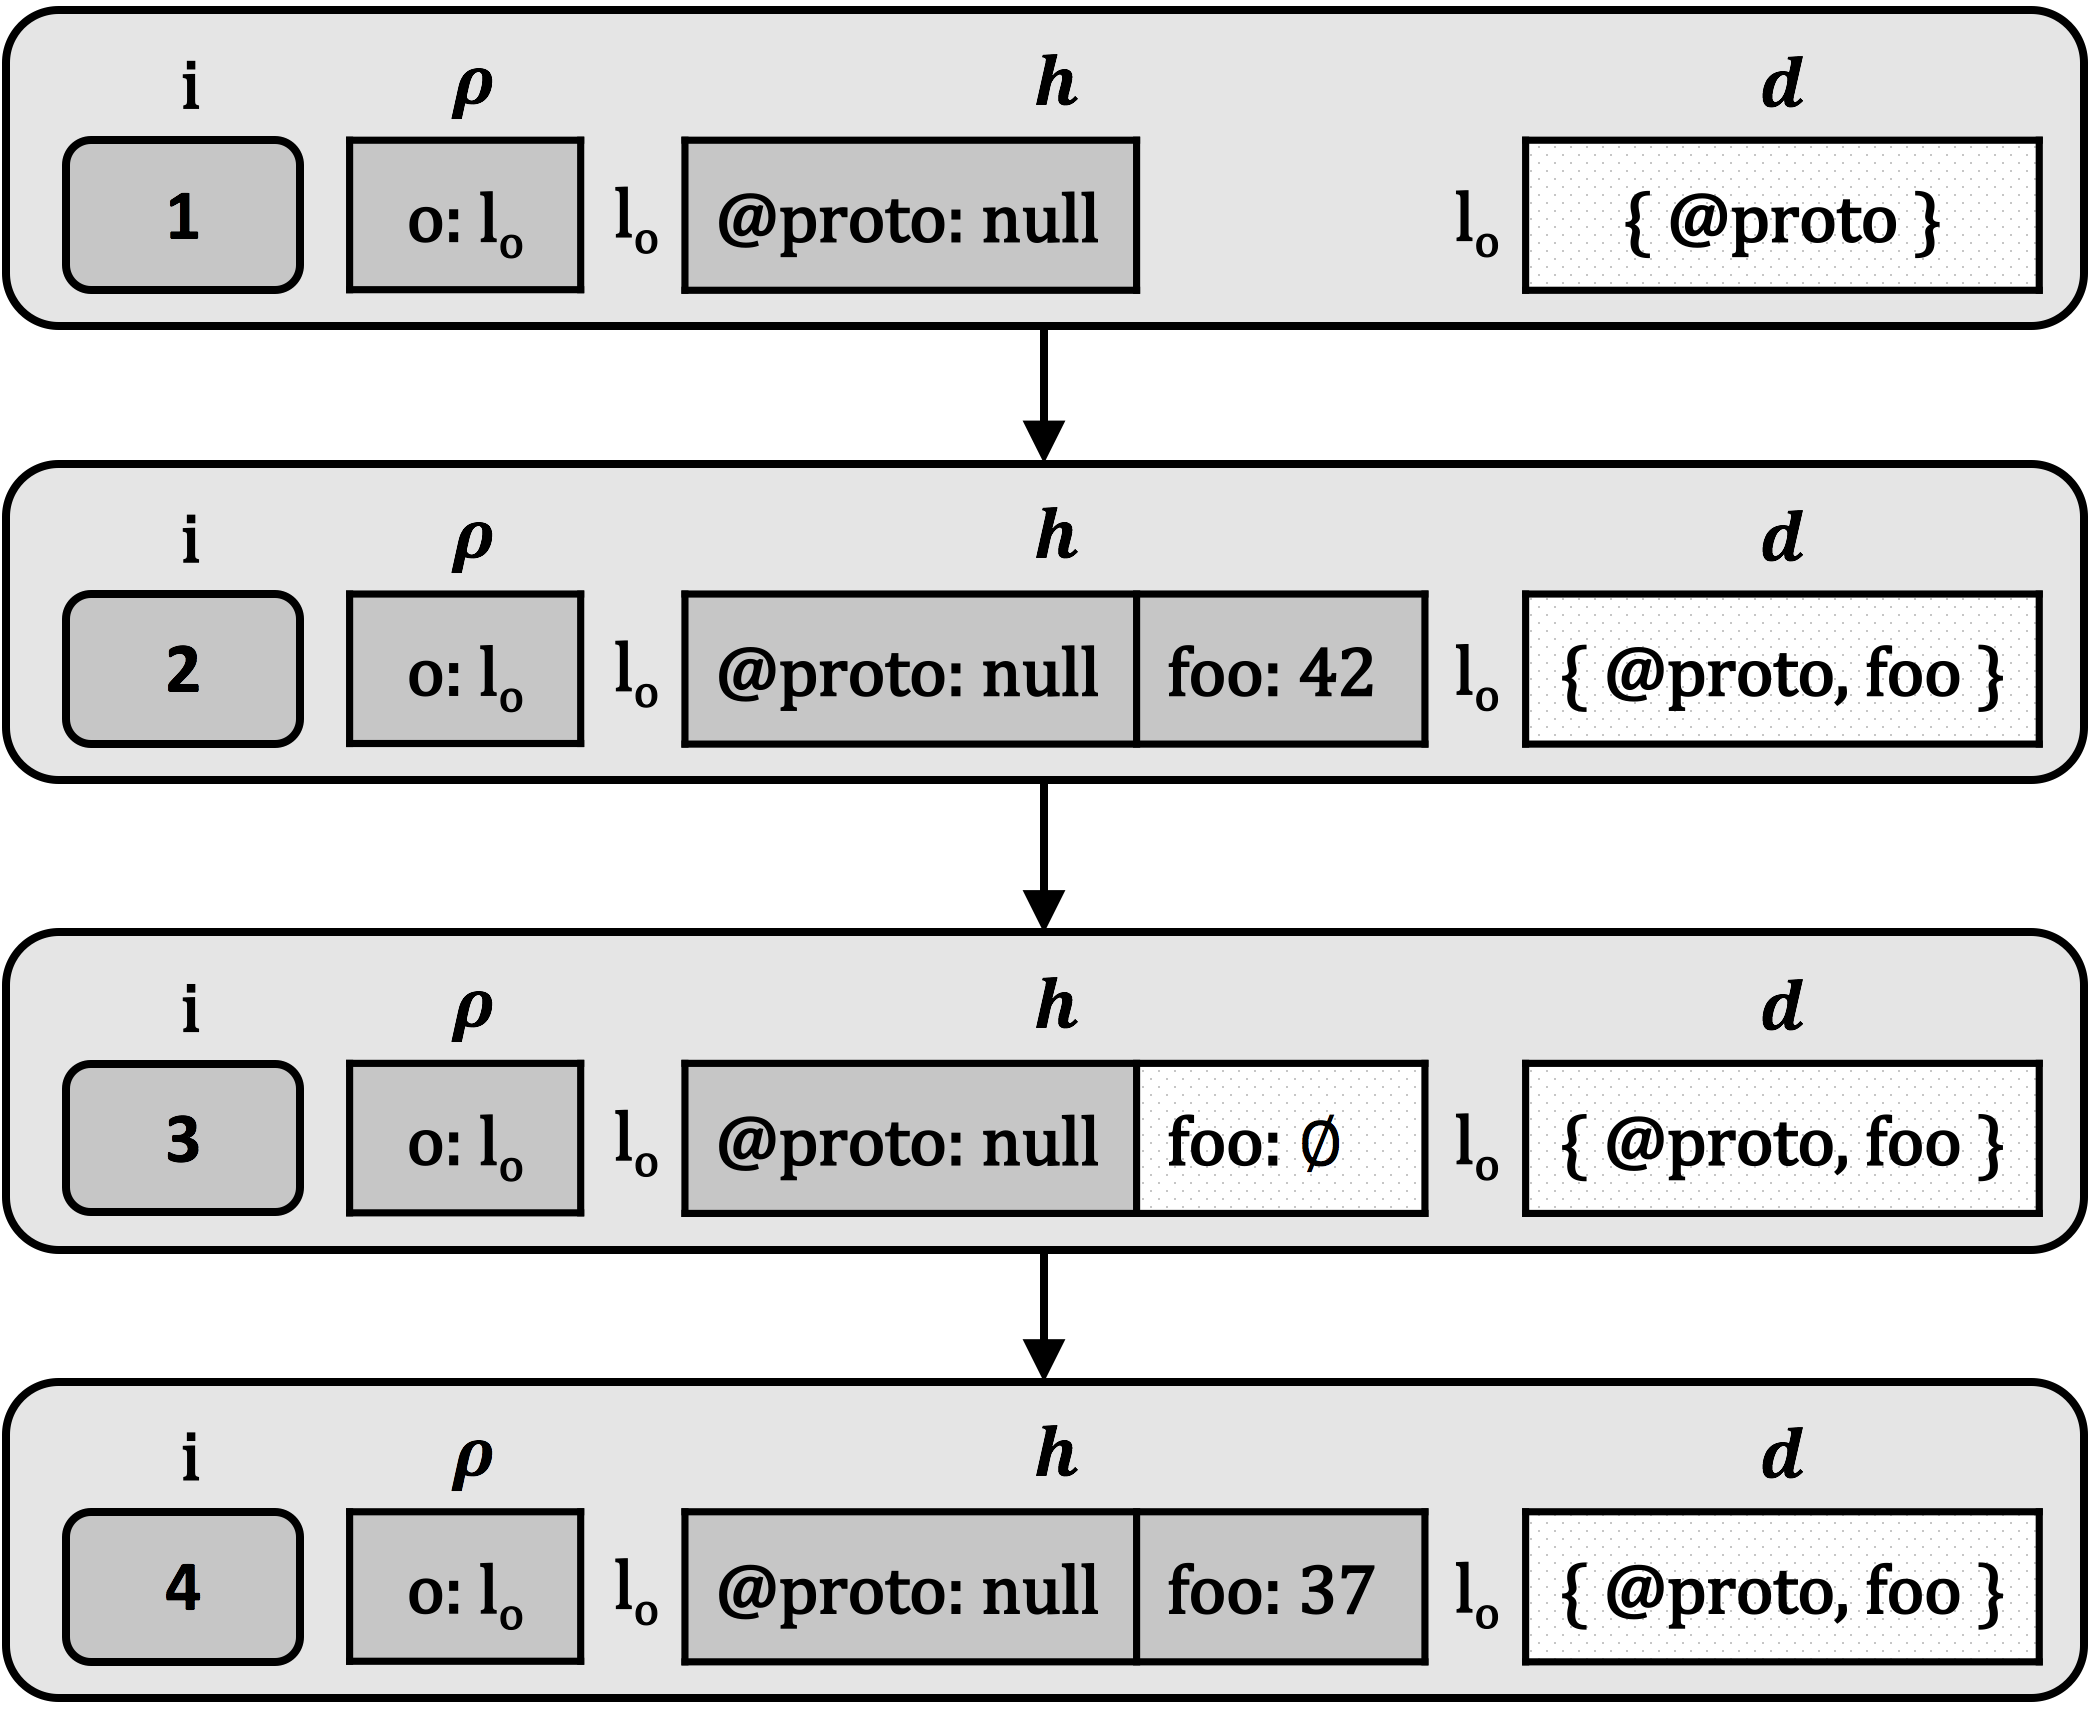
\includegraphics[width=0.28\textwidth]{figures/domaintable.png} \ & \ 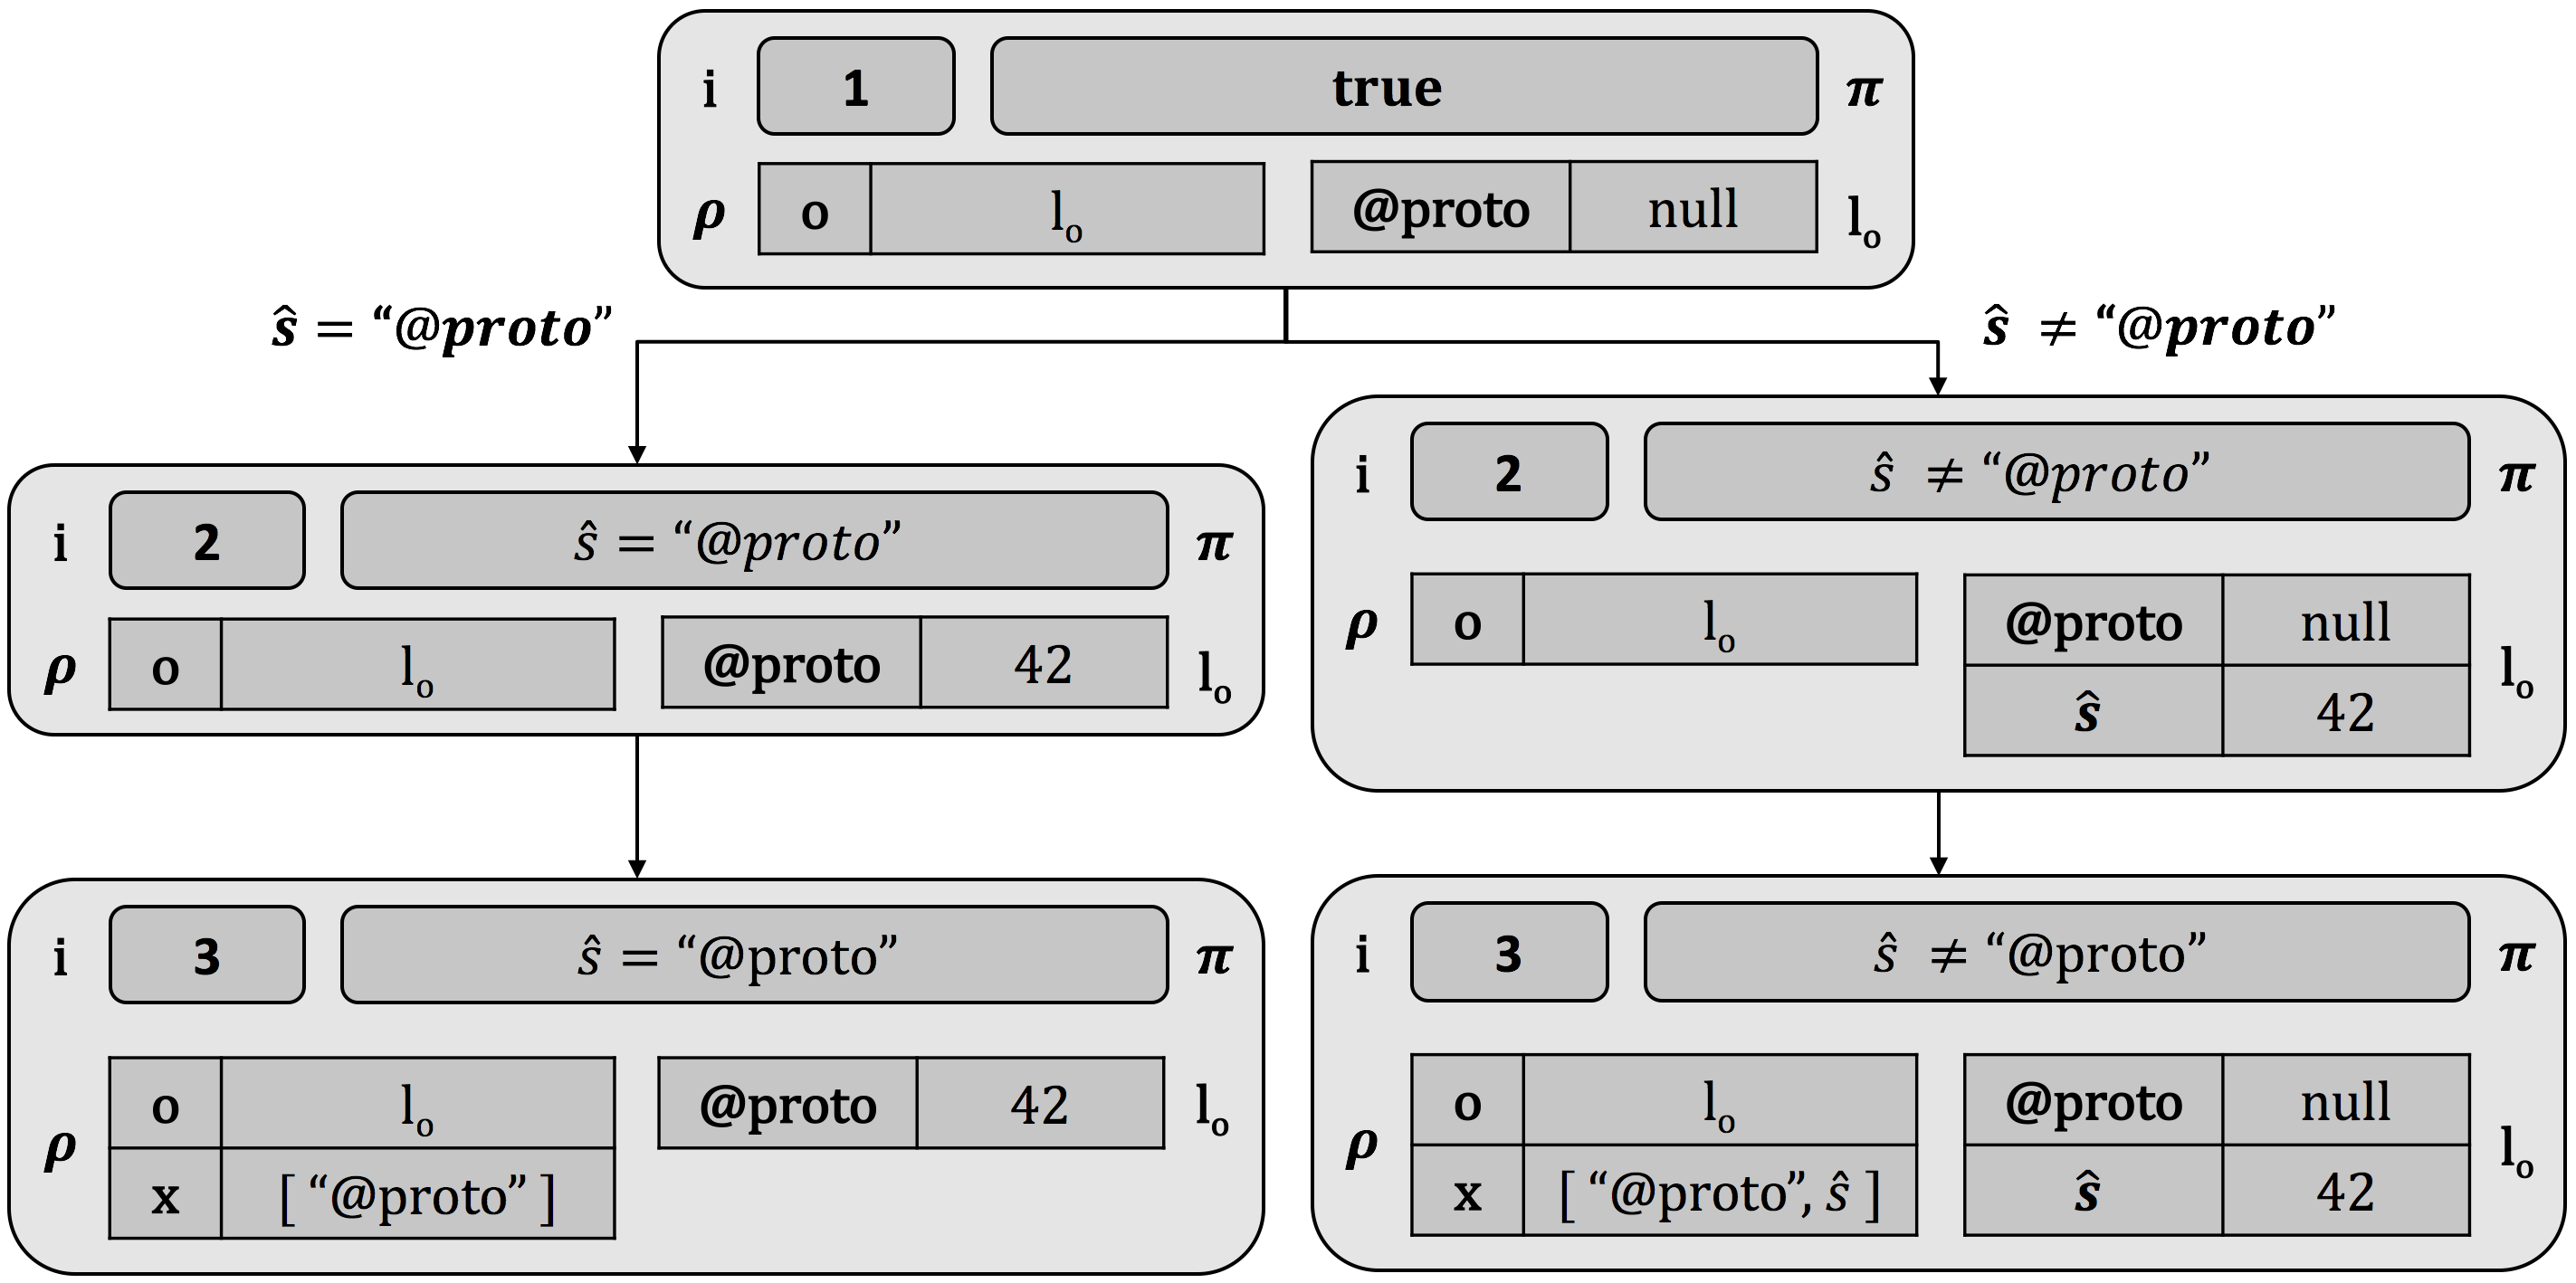
\includegraphics[width=0.59\textwidth]{figures/symbSemEx.png}
\end{tabular}
\vspace*{-0.3cm}
\caption{Execution traces: Instrumented GetCell (left); Symbolic branching (right)}
\label{fig:sexecexample}
\vspace*{-0.4cm}
\end{figure*}


As $\ival$ ranges over $\setext{\vals}{\none}$, the \textsc{Heap Update} rule may update the value of an object property to $\none$.  
In the concrete case, the corresponding rule would simply remove that property from the heap.  
 As an instrumented heap can contain $\none$-cells, the \textsc{GetDomain} rule has to filter out properties mapped to $\none$. 
 Furthermore, in order to apply this rule, one has to have full information about the object: all properties from $\idom(\loc)$ must be present in the heap. 
 %note how GetDomain collects all non-none properties of an object by inspecting both the heap and the domain table. 
%
Another difference between the two semantics is apparent in the rule \textsc{GetCell - Not Found}: while $\absgetcellrule{\instrumented}{\istate, \jsilexpr_1, \jsilexpr_2}{-, (-, -, \none)}$ 
means that one is certain that the object denoted by $\jsilexpr_1$ does not have the property 
denoted by $\jsilexpr_2$, $\absgetcellrule{\concrete}{\jstate, \jsilexpr_1, \jsilexpr_2}{-, (-, -, \none)}$ 
only means that this property does not exist in the current heap. %(and might be later framed on). 
%
%We note that the instrumented semantics does not evaluate symbolic variables.

 
 %As we inspect properties using GetCell, they .
 
 \myparagraph{Example: Frame revisited}
 In the rightmost column of Table~\ref{example:symb:states:vs:assertions}, we give the instrumented 
 execution of the frame example when
 the object at location $l_o$ is guaranteed not to have the property $\litstring{get}$. 
 Then, the  instrumented heap cannot be extended  with 
 the frame $(\loc_o, \litstring{get}) \mapsto 5$ as it overlaps with $(\loc_o, \litstring{get}) \mapsto \none$, meaning 
 that the illustrated frame bug cannot be replicated in the instrumented setting.  
 Also, if we remove $(\loc_o, \litstring{get}) \mapsto \none$ from the initial heap, 
 the instrumented execution will get stuck in the execution of line~$0$. 

\begin{wrapfigure}{R}{0.12\textwidth}
\vspace*{-0.35cm}
{\small
\hspace*{-0.5cm} $\mathtt{1\quad o := \jsilnew ()}$ \\[-0.06cm]
\hspace*{-0.5cm} $\mathtt{2\quad [o, "foo"] := 42}$ \\[-0.06cm]
\hspace*{-0.5cm} $\mathtt{3\quad \jsildelete(o, "foo")}$ \\ [-0.06cm]
\hspace*{-0.5cm} $\mathtt{4\quad [o, "foo"] := 37}$ 
}
\vspace*{-0.4cm}
%{\hspace*{-1cm}{\mbox{\caption{\jsil Example 1\label{jsil:example:frame}}}}}
\end{wrapfigure}

\myparagraph{Example: Instrumented GetCell}
To better understand the interaction between GetCell, the heap, and the domain table, consider the 
 program on the right and its execution trace in Figure~\ref{fig:sexecexample} (left). When executing the first property assignment, following the abstract \textsc{Property Assignment} rule, we must call $\getcell(\mathtt{o, "foo"})$ to obtain the current value of the property. As the property is not in the heap, we are in the \textsc{Not Found} case of GetCell. The domain is extended with $\mathtt{"foo"}$, and the heap is extended with the none-cell $\mathtt{(\loc_o, "foo")} \mapsto \none$, whose value is then updated to 42 by the heap update. After the deletion, its value is reset to $\none$. The following property assignment will again call $\getcell(\mathtt{o, "foo"})$, but this time, we will be in the \textsc{Found} case of GetCell, as the property is in the heap.
In a nutshell, GetCell ensures that all inspected properties, both present and absent, are represented in the heap.

%\jfs{
%\begin{itemize}
%  \item An example to explain the domain and how it interacts with the none-fields
%\end{itemize}
%}



\myparagraph{Formal Guarantees}
Theorem~\ref{teo:frame:property} states that the \jsil instrumented semantics observes the 
frame property. Lemma~\ref{lemma:instrumented:semantics} relates the instrumented 
semantics with the concrete semantics via an erasure function  $\interpret{\instconc}{}$. Informally, $\interpret{\instconc}{}(\istate)$
denotes the concrete state obtained by erasing negative information in $\istate$ (i.e.~  
$\none$-cells and domain information). 
Lemma~\ref{lemma:instrumented:semantics} states that if a given execution 
goes through in the instrumented semantics, then its concretisation (given by $\interpret{\instconc}{}$) 
goes through in the concrete semantics. %All proofs can be found in the Appendix.
For $\istate = (\iheap, \idom, \store)$, we write $\istate \dunion \iheap'$ to denote $(\iheap \dunion \iheap', \idom, \store)$.

\begin{theorem}[Frame Property - Instrumented Semantics]\label{teo:frame:property}
\hspace*{-0.28cm}$$
\transabssemrule{\istate, \cs, i}{\istate', \cs', j}{\mode}{\mode'}{\instrumented}\Rightarrow
        \transabssemrule{\istate \dunion \iheap_f, \cs, i}{\istate' \dunion \iheap_f, \cs', j}{\mode}{\mode'}{\instrumented} 
$$
\end{theorem}

\begin{lemma}[Transparency for Instrumentation]\label{lemma:instrumented:semantics}
$$
\hspace*{-0.22cm}
\transabssemrule{\istate, \cs, i}{\istate', \cs', j}{\mode}{\mode'}{\instrumented} \Rightarrow \transabssemrule{\interpret{\instconc}{}(\istate), \cs, i}{\interpret{\instconc}{}(\istate'), \cs', j}{\mode}{\mode'}{\concrete} 
$$
\end{lemma}



%
%\begin{display}{Instrumented State Interpretation}
%{\scriptsize 
%\begin{mathpar}
%\inferrule[Symbolic Heaps]{}{
%\interpret{\instconc}{}(\hemp) \semeq \hemp
%\quad
%\frac{
%   \heap = \hcell{\loc}{p}{\val}
%}{
%\interpret{\instconc}{}(\hcell{\loc}{p}{\val}) \semeq  \heap
%}
%\quad
%  \interpret{\instconc}{}(\hcell{\loc}{p}{\none}) \semeq \hemp }
%\quad
%\frac{
%  \begin{array}{c}
%   \interpret{\instconc}{}(\iheap_i) = \heap_i, \hdom_i \mid_{i =1,2} \\
%   \heap = \heap_1 \dunion \heap_2
%  \end{array}
%}{
%\interpret{\instconc}{}(\iheap_1 \dunion \iheap_2) \semeq  \heap
%}
%\qquad
%\inferrule[Symbolic States]{
%    \interpret{\instconc}{}(\iheap) = \heap
%}{
%\interpret{\instconc}{}(\iheap, \idom, \store) \semeq (\heap, \store)
%}
%\end{mathpar}}
%\end{display}




\vspace*{-0.2cm}
\subsection{\jsil Symbolic Semantics}\label{subsec:symb:semantics}

We obtain the \jsil symbolic semantics by lifting the \jsil instrumented semantics to the symbolic level, following standard approaches~\cite{Rosette1}.
This lifting, however, is easier for us to achieve because we only need to instantiate the abstract semantics, rather than re-examine every command of the language.

We instantiate the abstract values to \emph{symbolic expressions}, $\sexpr \in \sexprs$, defined as follows: 
$\sexpr \triangleq \val \mid \svar \mid \unoper\ \sexpr \mid \sexpr \binoper \sexpr$. 
For clarity, we use $\sexprp$ for symbolic expressions denoting property names, and $\sexprv$ for symbolic
expressions denoting arbitrary values. 


A \emph{symbolic state}, $\sstate = (\sheap, \sdom, \sstore, \pc)$, consists of a 
symbolic heap~$\sheap$, a symbolic domain $\sdom$, a symbolic store $\sstore$, and a path condition~$\pc$. 
The symbolic heap, symbolic domain, and symbolic store are obtained from their instrumented 
counterparts of~\S\ref{subsec:instrumented}, by replacing concrete values with symbolic expressions: for example,~a symbolic heap, $\sheap \in \sheaps : \slocs \partialmap \sexprs \partialmap \setext{\sexprs}{\none}$,
 maps pairs of object locations and symbolic expressions to symbolic expressions
extended with $\none$. 
%A symbolic store, $\sstore \in \sstores$, is a mapping from program variables 
%$\jvar \in \jvars$ to symbolic expressions.
%A symbolic location, $\sdom \in \sdoms$,  a partial function mapping object locations 
%to symbolic expressions. 
%The \emph{heap domain} maps object locations to set of properties that may be defined in the corresponding object.  
A \emph{path condition}~\cite{symb:exec:survey} is a first-order quantifier-free formula which
 accumulates constraints on the symbolic variables that direct 
the execution to the current symbolic state.
For clarity of presentation, we conflate \jsil logical values and logical values, as well as the \jsil logical operators and boolean logical operators.
%Alternatively, we could have \jsil logical expressions and logical expressions separately, together with a lifting function for converting the former to the latter. 
%simplifying both reasoning and~presentation. %, as a path condition is simply a \jsil symbolic boolean expression. 

We instantiate the abstract semantics for the symbolic case.  
%by providing the appropriate definitions for the required abstract functions, 
%focussing on the relevant definitions below. % (we omit those that coincide with the instrumented case). 
We write $\absbsemrule{\sstate, \bcmd}{\sstate'}{\symbolic}$ for the symbolic semantic 
judgement for basic commands and $\abssemrule{\sstate, \scs, i}{\sstate', \scs', j}{\mode}{\mode'}{\symbolic}$ 
for commands. Symbolic call stacks, $\scs$, differ from concrete stacks in that they contain symbolic stores.
For $\sstate = (\sheap, \sdom, \sstore, \pc)$, we write $\sstate \wedge \sexprb$ to denote $(\sheap, \sdom, \sstore, \pc \wedge \sexprb)$, 
$\sstate.\hpsel$ to denote $\sheap$, and $\sstate.\pcsel\!$ to denote $\pc$.

%Furthermore, we redefine \jsil expressions, $\pvsexpr \in \pvsexprs$ to take into account symbolic values
% as follows: $\pvsexpr \triangleq \val \mid \jvar \mid \svar \mid \unoper\ \pvsexpr \mid \pvsexpr \binoper \pvsexpr$.
%Extended \jsil expressions differ from symbolic expressions in that they can contain program variables.
%We extend heaps, stores, and call stacks with symbolic expressions, obtaining symbolic 
%heaps, stores, and call stacks, respectively ranged over by $\sheap$, $\sstore$, and $\scs$.
% Therefore, an evaluation of a \jsil extended expression $\pvsexpr$ in a symbolic store $\sstore$ always yields a 
%symbolic expression $\sexpr$.

\vspace{2pt}
\begin{display}{Selected Symbolic Semantics Rules}
\text{
{\scriptsize
\begin{mathpar} 
% \inferrule[\textsc{Expression Evaluation}]
%  {}{
%        {\begin{array}{c}
%           \evalexpr{\symbolic}(\sstore, \val) = \val  \\[2pt]
%  	   \evalexpr{\symbolic}(\sstore, \jvar) = \sstore(\jvar)  
%        \end{array}} \quad
%	%
%	\frac{
%		\sexprv =  \evalexpr{\symbolic}(\sstore, \jsilexpr) \quad
%		\sexprv' = \left\{ {\begin{array}{l}
%		      \semop{\ominus} (\sexprv) \ \text{if } \sexprv \in \vals \\
%		      \ominus \sexprv                   \ \ \ \text{  otherwise}
%		 \end{array}} \right. 
%	  }{
%	    \evalexpr{\symbolic}(\sstore, \ominus \jsilexpr) = \sexprv'
%	  } \qquad
%	  %
%	  \frac{
%	     \begin{array}{c}
%	         \sexprv_1 = \evalexpr{\symbolic}(\sstore, \jsilexpr_1) \\[2pt]
%	         \sexprv_2 = \evalexpr{\symbolic}(\sstore, \jsilexpr_2)  
%	     \end{array}    
%	     \quad 
%	     \sexprv' = \left\{ {\begin{array}{l}
%		      \semop{\oplus} (\sexprv_1, \sexprv_2) \ \text{if } \sexprv_1, \sexprv_2 \in \vals \\
%		      \sexprv_1 \oplus \sexprv_2      \  \ \ \text{  otherwise}
%		 \end{array}} \right. 
%	  }{\evalexpr{\symbolic}(\sstore, \jsilexpr_1 \oplus \jsilexpr_2) = \sexprv'}}
%\\
%  \inferrule[\textsc{GetDomain}]
%   { 
%        \evalexpr{\symbolic}(\sstore, \jsilexpr) = \sloc
%      \quad
%       \sheap = \sheap' \, \uplus \, \big((\sloc, \sexprp_i) \mapsto \sexprv_i \big)\mid_{i = 0}^m  
%        \\\\
%        %
%          (\sloc,-) \notin \domain (\sheap')  
%        \quad
%         \pc \vdash \jsilset{\sexprp_1, ..., \sexprp_m} = \sdom(\sloc)
%         \\\\
%        \forall_{0 \leq i \leq n} \, \sexprv_i \neq \none 
%         \quad 
%           \forall_{n < i \leq m} \, \sexprv_i = \none 
%   }{  \absgetdomainfun{\symbolic}((\sheap, \sdom, \sstore, \pc), \jsilexpr) \semeq \jsilset{\sexprp_1, ..., \sexprp_n}}
%  \and
 % 
     \inferrule[\textsc{GetCell - Not Found}]
   { 
         \evalexpr{\symbolic}(\sstore, \jsilexpr_1) = \sloc
        \quad 
        \evalexpr{\symbolic}(\sstore, \jsilexpr_2) = \sexprp
      \quad
        \sheap' = \sheap \dunion ((\sloc, \sexprp) \mapsto \none)
       \quad
       \sdom' = \sdom[\sloc \mapsto \sdom(\sloc) \cup \jsilset{\sexprp}]
   }{  \absgetcellrule{\symbolic}{(\sheap, \sdom, \sstore, \pc), \jsilexpr_1, \jsilexpr_2}{(\sheap', \sdom', \sstore,  {\color{blue}\pc \, \wedge \, \sexprp \not\in \sdom(\sloc)}), (\sloc, \sexprp, \none)}}
  %
  \\
  %
    \inferrule[\textsc{GetCell - Found}]
   { 
         \evalexpr{}(\sstore, \jsilexpr_1) = \sloc
        \quad 
        \evalexpr{}(\sstore, \jsilexpr_2) = \sexprp
      \\\\
       \sheap = - \, \uplus \, (\sloc, \sexprp') \mapsto \sexprv
        \quad
        %
       %\pc \not\vdash \sexprp' \neq \sexprp 
       %\quad 
       \sstate' = (\sheap, \sdom, \sstore, {\color{blue} \pc \wedge (\sexprp = \sexprp')})
   }{  \absgetcellrule{\symbolic}{(\sheap, \sdom, \sstore, \pc), \jsilexpr_1, \jsilexpr_2}{\sstate', (\sloc, \sexprp, \sexprv)}}
 %
%   \inferrule[\textsc{Store Update}]
%   { 
%         \sstate = (\sheap, \sdom, \sstore, \pc) 
%         \\\\
%         \sstore' = \sstore[\jvar \mapsto \val]
%         \\\\
%         \sstate' = (\sheap, \sdom, \sstore', \pc)
%   }{  \stupdt{\symbolic}(\sstate, \jvar, \val) = \sstate'  }
%   %
%   \and 
%       \inferrule[\textsc{Heap Update}]
%   { 
%         \sstate = (\sheap, \sdom, \sstore, \pc) 
%         \\\\ 
%         \sheap' = \sheap[(\sloc, \sexprp) \mapsto \sexprv]
%         \\\\
%         \sstate' = (\sheap', \sdom, \sstore, \pc)
%   }{  \hpupdt{\symbolic}(\sstate, (\sloc, \sexprp), \sexprv) = \sstate' }
%\\
%  %
%      \inferrule[\textsc{Store Selector}]
%   {}{  \stosel((-, -, \sstore, -)) =  \sstore}
   \quad 
       \inferrule[\textsc{Assume}]
   {  
         \sexprb = \evalexpr{\symbolic}(\sstate.\stosel, \jsilexpr)
   }{  \absassume{\symbolic}(\sstate, \jsilexpr) =  \sstate \, \wedge \, \sexprb }
   \\
    \inferrule[\textsc{Check Sat - True}]
   { 
   	\sexprb = \evalexpr{\symbolic}(\sstate.\stosel, \jsilexpr)
         \quad
         (\sstate.\pcsel \wedge \sexprb) \text{ SAT}
   }{  \abssat{\symbolic}(\sstate, \jsilexpr) = \jtrue}
 \qquad 
    \inferrule[\textsc{Check Sat - False}]
   { 
         \sexprb = \evalexpr{\symbolic}(\sstate.\stosel, \jsilexpr)
         \quad
         (\sstate.\pcsel \wedge \sexprb) \text{ UNSAT}
   }{  \abssat{\symbolic}(\sstate, \jsilexpr) = \jfalse} 
 \end{mathpar}}}
 \end{display}

\noindent Symbolic variables evaluate to themselves: $\evalexpr{s}(\svar) = \svar$. 
As they have meaning only in the symbolic semantics, they cannot be evaluated in the concrete/instrumented semantics (cf. Appendix). 
The GetCell of the symbolic semantics non-deterministically branches on the inspected property $\sexprp$ being equal to any of the properties of the object at location $\sexprl$ (\textsc{GetCell - Found}), and also on it \emph{not being} in the domain of the object, i.e.~being different from all of its properties (\textsc{GetCell - Not Found}). In all cases, the relevant information (highlighted in blue) is recorded in the path condition. This non-determinism contrasts with the concrete/instrumented semantics, where non-determinism occurs only in object~allocation. 
The \textsc{Assume} rule strengthens the path condition with the symbolic expression we are assuming to hold. The two SAT-check rules check satisfiability of a given expression under the current path condition. 

 

\begin{wrapfigure}{R}{0.12\textwidth}
\vspace*{0.1cm}
{\footnotesize
\hspace*{-0.55cm} $\mathtt{1\quad o := new\ ()}$ \\[-0.06cm]
\hspace*{-0.55cm} $\mathtt{2\quad o[\hat{s}] := 42};$ \\[-0.06cm]
\hspace*{-0.55cm} $\mathtt{3\quad x := getProps(o);}$ \\[-0.06cm]
\hspace*{-0.55cm} $\mathtt{4\quad assert\ (card \ x = 2)}$
}
\vspace*{-0.35cm}
\end{wrapfigure}


\myparagraph{Example: Symbolic Branching}
To get a better intuition of the symbolic execution, observe the code snippet on the right and its symbolic execution in Fig.~\ref{fig:sexecexample} (right). 
This code: 
        \dtag{1}~creates a new object~\jsinline|o|;
	\dtag{2}~assigns 42 to the symbolic property $\hat{\mathtt{s}}$ of~\jsinline|o|; 
	\dtag{3}~collects all the properties of $\mathtt{o}$; and
	\dtag{4}~asserts that $\mathtt{o}$ has two properties in the end. 
	     The last assertion will produce a failing symbolic execution.
%
%To understand why, consider the symbolic execution of this program given in Figure~\ref{fig:sexecexample} (right).
%
The key insight is that the symbolic execution branches when executing the property assignment (line~2).
% 
More concretely, the symbolic execution can either use the rule \prooflab{GetCell - Found}, when 
the inspected property coincides with one of the object's existing properties ({\small$\hat{s} = \mathtt{``@proto"}$}), 
or the rule \prooflab{GetCell - Not Found}, when the inspected property is different from all of the 
object's existing properties ({\small $\hat{s} \neq \mathtt{``@proto"}$}). 
%
In the left branch, $\mathtt{o}$ has only a single property {\small$\mathtt{``@proto"}$} (that gets updated to 42), whereas
in the right branch, it has two properties, {\small$\mathtt{``@proto"}$} and $\hat{s}$. 
%
Therefore, the assert command fails in the left branch and the symbolic execution  produces the concrete counter-model 
{\small$\hat{s} = \mathtt{``@proto"}$}.

%
% is to branch on the targeted property of the object (in our case, the symbolic property $\hat{s}$ of object at location $\mathtt{l_o}$) being equal to any one or none of the already existing properties of the object (in our case, we have only $\mathtt{``@proto"}$), adding the appropriate equalities and/or inequalities to the path condition, and proceeding with the symbolic execution for all obtained branches. In this case, this means that the symbolic execution will branch on whether or not $\hat{s} = \mathtt{``@proto"}$. We obtain two symbolic states, shown in the second row of Figure \ref{fig:sexecexample}. The left branch corresponds to the (\textsc{Found}) case, when $\hat{s} = \mathtt{``@proto"}$: this equality is added to the path condition and the value of the property $\mathtt{``@proto"}$ is updated to 42. In the right branch, we have that $\hat{s} \neq \mathtt{``@proto"}$ (\textsc{Not Found}), hence object $\mathtt{o}$ has two properties: $ \mathtt{``@proto"}$, with value $\jnull$; and $\hat{s}$, with value 42.
%We start from an empty heap, empty domain, empty store, and path condition $\jtrue$: 
%$\sstate_0 = \tuple{\hemp, \demp, \storeemp, \jtrue}$. After the execution of the first command, $\mathtt{o := new\ ()}$, using the \textsc{Basic Command} and \textsc{Object Creation} rules, we get to the state {\small $\sstate_1 = \tuple{\{ \mathtt{l_o : \{ ``@proto" : null} \} \}, \mathtt{l_o : \{ ``@proto"} \} \}, \{ \mathtt{o : l_o} \} , \jtrue}$}, illustrated at the top of Figure~\ref{fig:sexecexample}.
%The next command to be executed is the property assignment $\mathtt{o[\hat{s}] := 42}$. The semantic rule for \textsc{Property Assignment} makes use 
%of the abstract function \textsc{GetCell}. 
%There are two potential \textsc{Get Cell} rules (\textsc{Not Found} and \textsc{Found}), and in our case, both of them are applicable. 
%The execution then continues in both branches with the property collection command $\mathtt{x := getFields(o)}$, which assigns the set of properties of the object $\mathtt{o}$ to the variable~$\mathtt{x}$ (last row of Figure~\ref{fig:sexecexample}). Finally, we execute $\mathtt{assert\ (card \ x = 2)}$, asserting that $\mathtt{o}$ has exactly two properties, which we observe to hold in the right branch, but not in the left.
%Therefore, following the \textsc{Assert - False} rule, we obtain a failing symbolic execution trace, from which a concrete counter-model can be derived ($\hat{s} = \mathtt{``@proto"}$).



%
%\begin{display}{Symbolic State Instrumented Interpretation}
%{\scriptsize 
%\begin{mathpar}
%\inferrule[Symbolic Heaps]{}{
%\interpret{\symbinst}{\senv}(\hemp) \semeq \hemp
%\qquad
%\frac{
%  \begin{array}{c}
%   l = \interpret{\symbconc}{\senv}(\sexprl) \quad 
%    p =  \interpret{\symbconc}{\senv}(\sexprp) \\
%    v =  \interpret{\symbconc}{\senv}(\sexprv) \quad 
%    \heap = \hcell{l}{p}{v}
%  \end{array}
%}{
%\interpret{\symbinst}{\senv}(\hcell{\sexprl}{\sexprp}{\sexprv}) \semeq  \heap
%}
%\qquad
%\frac{
%  \begin{array}{c}
%   l = \interpret{\symbconc}{\senv}(\sexprl) \quad 
%   p = \interpret{\symbconc}{\senv}(\sexprp)  \\ 
%      \heap = \hcell{l}{p}{\none}
%    \end{array}
%}{
%  \interpret{\symbinst}{\senv}(\hcell{\sexprl}{\sexprp}{\none}) \semeq \heap
%}
%\qquad
%\frac{
%  \begin{array}{c}
%   \interpret{\symbconc}{\senv}(\sheap_i) = \iheap_i, \hdom_i \mid_{i =1,2} \\ 
%   \iheap = \iheap_1 \dunion \iheap_2 
%   \end{array}
%}{
%\interpret{\symbinst}{\senv}(\sheap_1 \dunion \sheap_2) \semeq \iheap
%}}
%\\
%\inferrule[Symbolic Domains]
%{
%   \idom(\loc) = \val  \iff  \exists \sexprl \in \domain(\sdom) \, . \,  \loc = \interpret{\symbconc}{\senv}(\sexprl) \, \wedge \, \val = \interpret{\symbconc}{\senv}(\sdom(\sexprl))
%}{
%\interpret{\symbinst}{\senv}(\sdom) \semeq \idom
%}
%\and
%\inferrule[Symbolic States]{
%    \sstate = (\sheap, \sdom, \sstore, \pc) 
%    \quad 
%    \interpret{\symbinst}{\senv}(\sheap) = \iheap
%   \quad
%    \interpret{\symbinst}{\senv}(\sdom) = \idom
%    \\\\
%    \interpret{\symbconc}{\senv}(\sstore) = \store 
%    \quad
%    \interpret{\symbconc}{\senv}(\pc) = \jtrue 
%}{
%\interpret{\symbinst}{\senv}(\sstate) \semeq (\iheap, \idom, \store)
%}
%\end{mathpar}}
%\end{display}

\newcommand{\shorthand}{\sortstyle{I}_\senv}

\myparagraph{Formal Guarantees}
We relate the symbolic semantics to the instrumented semantics using 
\emph{symbolic environments}, $\senv : \svars \rightharpoonup \vals$, mapping 
symbolic variables to concrete values. 
A symbolic environment is \emph{well-formed} if it preserves types (e.g.~symbolic strings are mapped to strings). In the following, we  
assume well-formed symbolic environments. 
%
Given a symbolic environment $\senv$, we use $\shorthand(\sexpr)$ to denote the
interpretation of the symbolic expression $\sexpr$ under $\senv$, with the key case
being the one for symbolic variables: $\shorthand(\svar) = \senv(\svar)$. In the
standard way, we extend
$\shorthand$ to symbolic heaps, symbolic domains, symbolic stores, symbolic call stacks,
as well as programs. We use $\interpret{\symbinst}{\senv}(\sstate)$ to 
denote the instrumented state obtained by interpreting $\sstate$ under $\senv$:
$\interpret{\symbinst}{\senv}((\sheap, \sdom, \sstore, \pc)) = (\shorthand(\sheap), \shorthand(\sdom), \shorthand(\sstore))$ if $\shorthand(\pc) = \jtrue$; and is undefined otherwise.

Theorem~\ref{lemma:soundness:jsil:symb:exe:instrumented:instrumented} states 
that, given a symbolic trace, $\prog : \transabssemrule{\sstate, \scs, i}{\sstate', \scs', j}{\mode}{\mode'}{\symbolic}$,
 and an instrumented state in the interpretation of $\sstate$ \emph{filtered by the final 
 path condition}, there is an instrumented trace that will produce a final instrumented state 
 in the interpretation of the final symbolic state. 
 We use the final path condition $\sstate'.\pcsel$ when picking the initial 
 instrumented state because we only care about the initial instrumented states for which 
the instrumented execution follows the same path as the symbolic execution. 

%The soundness theorem (Theorem~\ref{teo:soundness:jsil:symb:exe}) states that if we have a symbolic trace captured by 
%$\symbtranstrans[\prog][\mode][\mode']{\sheap, \sstore, i, \pc}{\sheap', \sstore', i', \pc'}[\sctx][\sctx']$ 
%and a concrete state $(\heap, \store, \ctx)$ with a symbolic environment~$\senv$
%in the models of the initial symbolic state under 
%the final path condition $\pc'$, and $\senv$ concretises all symbolic variables of the program $\prog$, then there exists a concrete symbolic state $(\heap', \store', \ctx')$ 
%that is in the models of the final symbolic state under $\pc'$ with the same symbolic environment~$\senv$, such that: 
%$\semtranstrans[\symbeval{\prog}{\senv}][\mode][\mode']{\heap, \store, i}{\heap', \store', i'}[\ctx][\ctx']$. 


\begin{theorem}[Bounded Soundness]\label{lemma:soundness:jsil:symb:exe:instrumented:instrumented}
\vspace*{-0.1cm}
$$
\begin{array}{l}
\prog : \transabssemrule{\sstate, \scs, i}{\sstate', \scs', j}{\mode}{\mode'}{\symbolic} \ \wedge \ \istate = \interpret{\symbinst}{\senv}(\sstate \, \wedge \, \sstate'.\pcsel) \\ \quad \ \wedge \ \cs = \shorthand(\scs) \ \Rightarrow \ \exists \, \istate', \cs' \, . \, 
        \shorthand(\prog) : \transabssemrule{\istate, \cs, i}{\istate', \cs', j}{\mode}{\mode'}{\instrumented} \\ \quad \quad \quad \quad  \quad \quad \quad \quad  \quad \quad
             \ \wedge \ \istate' = \interpret{\symbinst}{\senv}(\sstate')  \ \wedge \ \cs' = \shorthand(\scs')
\end{array}
$$
\end{theorem}



\vspace*{-0.25cm}
\subsection{Linking the Semantics}\label{sex:formal:guarantees}

The last step of our methodology consists of linking the symbolic semantics to the concrete semantics in a way that describes the frames that can be safely added to the initial state.  
In other words, the interpretation of symbolic states needs to describe both the concretisation of that state and the safe frames for that concretisation. 

Below, we give the formal interpretation of symbolic states, 
$\interpret{\symbconc}{\senv}(\sstate)$. This interpretation denotes a set of pairs of the form $(\jstate, \heap_f)$,
where $\jstate$ is the concrete state obtained from $\sstate$ using $\senv$, and $\heap_f$ is
a concrete heap frame that can be safely added to $\jstate$, meaning that it does not overlap with either the positive or the negative resource captured by~$\sstate$. The positive resource is collected by $\interpret{\symbconc}{\senv}(\sheap)$ (its first component), whereas the negative resource is collected by $\interpret{\symbconc}{\senv}(\sheap)$ (its second component) and by $\interpret{\symbconc}{\senv}(\sdom)$. 
Here, we represent the negative resource as a set $\hdom$ of pairs of the form $(\loc, p)$ capturing the 
object properties that must not exist in the heap.


\smallskip
 \begin{display}{Symbolic State Interpretation}
{\scriptsize 
\begin{mathpar}
%
\inferrule[Empty Heap]{}{
\interpret{\symbconc}{\senv}(\hemp) \semeq \hemp, \emptyset
}
\qquad
\inferrule[Non-none Cell]{
%   l = \interpret{\symbconc}{\senv}(\sexprl) \quad 
%    p =  \interpret{\symbconc}{\senv}(\sexprp) \\\\
%    v =  \interpret{\symbconc}{\senv}(\sexprv)  \quad 
    \heap = \hcell{\shorthand(\sexprl)}{\shorthand(\sexprp)}{\shorthand(\sexprv)}
}{
\interpret{\symbconc}{\senv}(\hcell{\sexprl}{\sexprp}{\sexprv}) \semeq  (\heap, \emptyset)
}
\qquad
\inferrule[None Cell]{
%   l = \interpret{\symbconc}{\senv}(\sexprl) \quad 
%   p = \interpret{\symbconc}{\senv}(\sexprp)  \\\\
   \hdom = \jsilset{ (\shorthand(\sexprl), \shorthand(\sexprp) }
}{
  \interpret{\symbconc}{\senv}(\hcell{\sexprl}{\sexprp}{\none}) \semeq (\hemp, \hdom)
}
\\
\inferrule[Heap Composition]{
%   \interpret{\symbconc}{\senv}(\sheap_i) = h_i, \hdom_i \mid_{i =1,2} \\\\
   \heap = \interpret{\symbconc}{\senv}(h_1) \dunion \interpret{\symbconc}{\senv}(h_2) \\\\
   \hdom = \interpret{\symbconc}{\senv}(\hdom_1) \dunion \interpret{\symbconc}{\senv}(\hdom_2)
}{
f(\sheap_1 \dunion \sheap_2) \semeq (\heap, \hdom)
}
\qquad
\inferrule[Symbolic Domains]
{
  \hdom =  \left\{ (l, p) \mid 
                     {
                         \sexprl \in \domain(\sdom) \, \wedge \, l = \shorthand(\sexprl)  
                              \, \wedge \, p \not\in \shorthand(\sdom(\sexprl))
                     } \right\}
}{
\interpret{\symbconc}{\senv}(\sdom) 
    \semeq \hdom 
}
\and
\inferrule[Symbolic States]{
    \sstate = (\sheap, \sdom, \sstore, \pc) 
    \quad 
   \interpret{\symbconc}{\senv}(\sheap) = \heap, \hdom_1
   \quad
   \interpret{\symbconc}{\senv}(\sdom) = \hdom_2
   \quad
   \shorthand(\sstore) = \store
    \quad 
    \shorthand(\pc) = \jtrue 
}{
\interpret{\symbconc}{\senv}(\sstate) \semeq \{ ((\heap, \store), \heap_f) \mid \domain(\heap_f) \cap (\domain(h) \cup \hdom_1 \cup \hdom_2) = \emptyset \} 
}
\end{mathpar}}
\end{display}

\smallskip
Theorem~\ref{teo:soundness:jsil:symb:exe} states the bounded soundness of the \jsil symbolic 
execution with respect to the concrete semantics. Moreover, this theorem quantifies over all possible 
frames, which is not the case for standard results in symbolic execution~\cite{saxena:sp:2010,li:fse:2014,koushik:fse:2015,wittern:icse:2018}, 
which do not establish frame resilience. 

%\pmax{Mention related work stronger.}
\vspace*{-0.1cm}
\begin{theorem}[Bounded Soundness + Frame Resilience]\label{teo:soundness:jsil:symb:exe}
$$
\begin{array}{l}
\prog : \transabssemrule{\sstate, \scs, i}{\sstate', \scs', j}{\mode}{\mode'}{\symbolic} 
    \\ \quad \wedge \ (\jstate, \heap_f) \in \interpret{\symbconc}{\senv}(\sstate \, \wedge \, \sstate'.\pcsel) \ \wedge \ \cs = \shorthand(\scs) \\ \qquad \implies \exists \, \jstate', \cs' \, . \,
        \shorthand(\prog) : \transabssemrule{\jstate \dunion \heap_f, \cs, i}{\jstate' \dunion \heap_f, \cs', j}{\mode}{\mode'}{\concrete} \\ \qquad \qquad \quad
               \wedge \ (\jstate', \heap_f) \in \interpret{\symbconc}{\senv}(\sstate')
               \ \wedge \ \cs' = \shorthand(\scs')
\end{array}
$$
\end{theorem}

The \emph{bug-finding} corollary (Corollary~\ref{bug:finding}) states that if 
we find a symbolic trace that results in a failed assertion, 
then there also exists a concrete execution for which that assertion fails.
The analysis is designed in such a way that there are no false positives: 
if we find a failing symbolic trace,
we can always instantiate its symbolic values to obtain a concrete counter-model for the 
failing assertion. %This is essential, as \cosette is primarily a \emph{bug-finding} tool.

\vspace*{-0.1cm}
\begin{corollary}[Bug-finding]\label{bug:finding}
$$
\begin{array}{l}
\prog : \transabssemrule{\sstate, \scs, i}{-, -, j}{\mode}{\bot}{\symbolic}  \\ \quad  
%
   \implies \  \exists \senv \, . \, (\jstate, -) \in \interpret{\symbconc}{\senv} \, \wedge \, 
          \shorthand(\prog) :  \transabssemrule{\jstate, \shorthand(\scs), i}{-, -, j}{\mode}{\bot}{\concrete} 
\end{array}
$$
\end{corollary}

%Finally, the \emph{verification} corollary (Corollary~\ref{corollary:verification})
%states that if we have symbolically explored all possible execution paths
%starting from a given symbolic state and call stack $(\sstate, \scs)$,  
%then the execution of the program starting from any concrete state in the models 
%of the initial symbolic state (under the initial path condition) will result in a final concrete state
%in the models of one of the final symbolic states (under its associated path condition).  
%As \cosette does not infer loop invariants, if a program contains loops that cannot be unrolled statically, we will never be in the case of the verification~corollary. 
%
%\vspace*{-0.1cm}
%\begin{corollary}[Verification]\label{corollary:verification}
%$$
%\begin{array}{l}
%\wedge_{k=1}^n \, \big( \transabssemrule{\sstate, \scs, i}{\sstate_k, \scs_k, j_k}{\mode}{\mode_k}{\symbolic}  \big)
%    \, \wedge \, \big( \sstate.\pcsel \vdash \vee_{k=1}^n \sstate_k.\pcsel \big)  \\  \quad
%    \, \wedge \, (\jstate, \cs, \heap_f) \in \interpret{\symbconc}{\senv}(\sstate, \scs)
%    \\ \qquad 
%%
%      \ \implies \ \exists l \in \overline{1, n}, \senv', \jstate', \cs' \, . \, 
%           \transabssemrule{\jstate, \cs, i}{\jstate', \cs', j_l}{\mode}{\mode_l}{\concrete} \\ \qquad \qquad \qquad
%           \, \wedge \, 
%           (\jstate', \cs', \heap_f) \in \interpret{\symbconc}{\senv'}(\sstate_l, \scs_l)
%\end{array}
%$$
%\end{corollary}

%
%The {\bf proofs} of all the results in this section, as well as all the complete definitions, are given in the Appendix.

%
%
%
%\begin{lemma}[Two-Level Symbolic Interpretation]\label{lemma:symb:interpretation}
%$$
%(\jstate, \cs, \heap_f) \in \interpret{\symbconc}{\senv}(\sstate, \scs) 
%   \iff 
%   \exists \, \istate, h_F \, . \, 
%         (\istate, \cs) = \interpret{\symbinst}{\senv}(\sstate, \scs)  
%          \ \wedge \   
%      \jstate = \interpret{\instconc}{}(\istate)
%      \ \wedge \
%      h_F \disjoint \istate.\hpsel
%$$
%\end{lemma}

\vspace*{-0.3cm}
\subsection{Implementation}\label{subsec:jsil:analysis:implementation}

Our three semantics for \jsil (\S\ref{subsec:concr}--\S\ref{subsec:symb:semantics}) are specifically designed with implementation in mind: one only needs to follow the rules, which are written operationally, modularly, and are syntax-directed. 

However, implementing the entailment engine required by the symbolic semantics and practically handling the state explosion problem~\cite{clarke:lpar:2008} is a challenging task. For this reason, we develop the first, proof-of-concept version of \cosette leveraging on 
\rosette~\cite{Rosette1,Rosette2}, a symbolic virtual machine that enables the development of solver-aided languages. \rosette extends Racket~\cite{racket} with symbolic values and first-order assertions over these values, and languages implemented in \rosette can make use of its solver-aided facilities. 

We implement the \emph{instrumented} \jsil interpreter of \S\ref{subsec:instrumented} in \rosette, obtaining a \jsil symbolic interpreter for free. We show that this symbolic interpreter is consistent with the symbolic semantics given in \S\ref{subsec:symb:semantics}, as described in \S\ref{sec:intro}.
%To make certain that this symbolic interpreter is consistent with the symbolic semantics of \S\ref{subsec:symb:semantics}, we systematically construct symbolic unit tests for each \jsil command, assuming the premises and asserting the conclusion of the appropriate rule of the symbolic semantics. For lack of space, more information on these tests is available in the Appendix.
We note that, as Rosette does not finitise the symbolic execution of loops branching on symbolic values~\cite{abstract:symbolic:exec}, the user must specify the maximum allowed number of such branchings. Once that bound is reached, the symbolic execution~stops.

\vspace*{-0.2cm}
\subsection{Lifting the results to JavaScript}
\label{subsec:liftmejs1}

All the results presented in this section lift to JavaScript in a straightforward way.
One simply has to: 
\dtag{1} extend JavaScript with constructs for creating symbolic values and 
asserting and assuming first-order formulae; and
\dtag{2} compile JavaScript to \jsil using a correct compiler. 
Here, we make use of \jstojsil~\cite{javert}, a thoroughly tested and formally validated compiler from 
JavaScript to \jsil.

To illustrate the lifting, we restate Corollary~\ref{bug:finding} for JavaScript.
Given a JavaScript symbolic state, $\sstate_\jssubscript$, and program $\jstmt$, we translate 
both the state and program to \jsil, obtaining a \jsil symbolic state and context, $(\sstate, \scs)$,
and a \jsil program $\prog$.  
We then run the obtained \jsil program in the symbolic semantics. 
If there is an assertion failure at the \jsil level, then, by the correctness of \JSComp, 
that failure is guaranteed to exist at the JavaScript level as well. Formally: 
$$
\begin{array}{l}
\compile(\sstate_\jssubscript) = (\sstate, \scs) \, \wedge \, \compile(\jstmt) = \prog \, \wedge \, 
  \prog :  \transabssemrule{\sstate, \scs, i}{-, -, j}{\mode}{\bot}{\symbolic}  \\ \quad 
      \ \implies \ \exists \, \jstate_\jssubscript \, . \, \transjssemrulebug{\jstate_\jssubscript', \jstmt}
\end{array}
$$


%\begin{corollary}[Bug-finding for JavaScript]\label{bug:finding:js}
%\end{corollary}

%\pmax{Zzzzzz, we may need more, possibly just in words.}
 
%
%To make use of the symbolic execution tool for \jsil, one needs to compile 
%
%
%
%We extend the syntax of JavaScript with 
%
%
%asserting and assuming first order propositional formulae. 
%
%and the following constructs: %(corresponding to JavaScript normal expressions): 
%\dtag{1} $\jsassert(\jslexpr)$, stating that whenever the \emph{assert} is reached, 
%$\jslexpr$ must evaluate to $\jtrue$; 
%\dtag{2} $\jsassume(\jslexpr)$, stating that we \emph{assume} $\jslexpr$ to hold along the
%current program path; 
%\dtag{3} $\jssymbstring()$, for creating a fresh symbolic string; and
%\dtag{4} $\jssymbnumber()$, for creating a fresh symbolic number. 
%The \emph{assert} and \emph{assume} constructs expect as an argument 
%a logical expression. 


